\documentclass[semifinal]{cpecmu}

%% This is a sample document demonstrating how to use the CPECMU
%% project template. If you are having trouble, see "cpecmu.pdf" for
%% documentation.

\projectNo{S809-2}
\acadyear{2025}

\titleTH{เปเปอร์เกรดเดอร์: แพลตฟอร์มสำหรับการตรวจใบงานแบบกระดาษ}
\titleEN{PaperGrader: A platform for grading paper-based assignments}

\author{นายคณพัฒน์ ประเพชร}{Kanaphat Prapet}{630612095}
\author{นายจิรายุ จิตรเปรม}{Jirayu Jitprem}{630612096}
\author{นายวิศรุต สาดา}{Wisarut Sada}{630612110}

\cpeadvisor{dome}
\cpecommittee{navadon}
\cpecommittee{trasapong}

%% Some possible packages to include:
\usepackage[final]{graphicx} % for including graphics

%% Add bookmarks and hyperlinks in the document.
\PassOptionsToPackage{hyphens}{url}
\usepackage[colorlinks=true,allcolors=Blue4,citecolor=red,linktoc=all]{hyperref}
\def\UrlLeft#1\UrlRight{$#1$}

%% Needed just by this example, but maybe not by most reports
\usepackage{afterpage} % for outputting
\usepackage{pdflscape} % for landscape figures and tables. 

%% Some other useful packages. Look these up to find out how to use
%% them.
% \usepackage{natbib}    % for author-year citation styles
% \usepackage{txfonts}
% \usepackage{appendix}  % for appendices on a per-chapter basis
% \usepackage{xtab}      % for tables that go over multiple pages
% \usepackage{subfigure} % for subfigures within a figure
% \usepackage{pstricks,pdftricks} % for access to special PostScript and PDF commands
% \usepackage{nomencl}   % if you have a list of abbreviations

%% if you're having problems with overfull boxes, you may need to increase
%% the tolerance to 9999
% \tolerance=9999

\bibliographystyle{plain}
% \bibliographystyle{IEEEbib}

% \renewcommand{\topfraction}{0.85}
% \renewcommand{\textfraction}{0.1}
% \renewcommand{\floatpagefraction}{0.75}

%% Example for glossary entry
%% Need to use glossary option
%% See glossaries package for complete documentation.
\ifglossary
  \newglossaryentry{lorem ipsum}{
    name=lorem ipsum,
    description={derived from Latin dolorem ipsum, translated as ``pain itself''}
  }
\fi

%% Uncomment this command to preview only specified LaTeX file(s)
%% imported with \include command below.
%% Any other file imported via \include but not specified here will not
%% be previewed.
%% Useful if your report is large, as you might not want to build
%% the entire file when editing a certain part of your report.
% \includeonly{chapters/intro,chapters/background}

\begin{document}
\maketitle
\makesignature

\ifproject
\begin{abstractTH}
\sloppy \par
โครงงานนี้มีจุดประสงค์เพื่อพัฒนาแพลตฟอร์มสำหรับการตรวจใบงานแบบกระดาษในมหาวิทยาลัยเชียงใหม่ โดยแพลตฟอร์มที่พัฒนาขึ้นจะช่วยลดปัญหาที่เกิดจากกระบวนการตรวจและบันทึกคะแนนในปัจจุบัน ซึ่งเป็นกระบวนการที่ใช้เวลานานและซับซ้อน โดยเฉพาะการเปลี่ยนแปลงเกณฑ์คะแนนที่ต้องมีการคำนวณใหม่ซ้ำซ้อน แพลตฟอร์มที่พัฒนาจะมีฟังก์ชันที่ช่วยในการกำหนดเกณฑ์คะแนนที่ยืดหยุ่น รองรับการปรับเปลี่ยนได้ตามต้องการ รวมถึงการจัดการข้อมูลคะแนนอย่างเป็นระบบและสามารถติดตามผลการตรวจงานได้อย่างมีประสิทธิภาพ นอกจากนี้แพลตฟอร์มนี้ยังเป็นเครื่องมือสำหรับนักศึกษาในการติดตามคะแนนของใบงานและยื่นคำร้องขอตรวจคะแนนใหม่ได้เมื่อพบความผิดพลาด ผลจากการพัฒนาระบบนี้จะช่วยลดภาระการจัดเก็บและค้นหาใบงานในรูปแบบกระดาษของอาจารย์ รวมถึงลดความล่าช้าและความผิดพลาดจากการตรวจและบันทึกคะแนนในรูปแบบดั้งเดิม ทำให้การจัดการเอกสารและคะแนนเป็นไปอย่างมีประสิทธิภาพมากยิ่งขึ้น
\end{abstractTH}

\begin{abstract}
\par
The objective of this project is to develop a platform for grading paper-based assignments at Chiang Mai University. The proposed platform aims to address challenges in the current grading and score-recording processes, which are time-consuming and complex, particularly when changes to grading criteria require recalculations. The developed platform will feature flexible grading functions that accommodate adjustments as needed, along with systematic score management to efficiently track grading outcomes. Additionally, this platform serves as a tool for students to monitor their assignment scores and submit requests for regrading when errors are identified. The implementation of this system will reduce the burden of paper-based assignment storage and retrieval for instructors, decrease delays in the grading process, and minimize errors associated with traditional scoring and record-keeping. As a result, it will enhance the efficiency of document and score management.
\end{abstract}

\iffalse
\begin{dedication}
This document is dedicated to all Chiang Mai University students.

Dedication page is optional.
\end{dedication}
\fi % \iffalse

\begin{acknowledgments}
\par
โครงงานนี้จะไม่สามารถสำเร็จได้ถ้าไม่ได้ความกรุณาจาก ผศ. โดม โพธิกานนท์ อาจารย์ที่ปรึกษาโครงงาน ที่ได้สละเวลาความช่วยเหลือให้คำแนะนำและสนับสนุนในการทำโครงงานนี้ จนทำให้โครงงานเล่มนี้เสร็จ สมบูรณ์ไปได้
\acksign{2025}{10}{30}
\end{acknowledgments}%
\fi % \ifproject

\contentspage

\ifproject
\figurelistpage

\tablelistpage
\fi % \ifproject

% \abbrlist % this page is optional

% \symlist % this page is optional

% \preface % this section is optional


\pagestyle{empty}\cleardoublepage
\normalspacing \setcounter{page}{1} \pagenumbering{arabic} \pagestyle{cpecmu}

\chapter{\ifenglish Introduction\else บทนำ\fi}

\section{\ifenglish Project rationale\else ที่มาของโครงงาน\fi}
\qquad ปัจจุบันการตรวจใบงานแบบกระดาษและการบันทึกคะแนนลงในคอมพิวเตอร์ยังคงใช้เวลาที่นานและมีความซ้ำซ้อน โดยกระบวนการนี้มีความซับซ้อนในหลายลำดับ ยกตัวอย่างเช่น อาจารย์ในมหาวิทยาลัยเชียงใหม่ที่สอนหลายกระบวนวิชามีปริมาณกระดาษข้อสอบและ ใบงานจำนวนมาก เมื่อมีการเปลี่ยนแปลงเกณฑ์การให้คะแนน จึงจำเป็นต้องกลับมาตรวจและคำนวณคะแนนใหม่อีกครั้ง ทำให้กระบวนการนี้เกิดความล่าช้าและการให้คะแนนในรูปแบบใบงานที่เป็นกระดาษยังซับซ้อน  ต้องบันทึกคะแนนลงในระบบคอมพิวเตอร์หรือ 
แพลตฟอร์มอื่นและนำไปวิเคราะห์สถิติในภายหลัง  การจัดเก็บใบงานในรูปแบบกระดาษต้องใช้พื้นที่ในการจัดเก็บที่มาก และการค้นหาใบงานจะยิ่งยากหากมีปริมาณใบงานมาก นอกจากนี้ยังเสี่ยงต่อการสูญหาย และหากนักศึกษายื่นขอตรวจคะแนนใหม่ จำเป็นต้องค้นหาใบงานเพื่อตรวจซ้ำอีกรอบ 

\qquad แพลตฟอร์มสำหรับการตรวจใบงานแบบกระดาษ (PaperGrader) เป็นแพลตฟอร์มที่เป็นทางเลือกสำหรับอาจารย์ในมหาวิทยาลัยเชียงใหม่ ที่จะเข้ามาช่วยในเรื่องการกำหนดเกณฑ์คะแนนที่ซับซ้อน การปรับเปลี่ยนเกณฑ์คะแนนระหว่างการตรวจ นอกจากนี้ยังช่วยให้นักศึกษาในมหาวิทยาลัยเชียงใหม่ สามารถติดตามคะแนนของใบงานและสามารถมีการยื่นคำร้องขอเพื่อขอรับการตรวจคะแนนใหม่จากอาจารย์ผู้สอน

\section{\ifenglish Objectives\else วัตถุประสงค์ของโครงงาน\fi}
    \begin{enumerate}
        \item เพื่อพัฒนาแพลตฟอร์มในการตรวจใบงานแบบกระดาษ  ที่จะเข้ามาช่วยลดความล่าช้าในการให้คะแนน และปรับเปลี่ยนเกณฑ์คะแนนในภายหลังของใบงาน
        \item เพื่อช่วยให้ผู้สอนสามารถวิเคราะห์สถิติคะแนน เพื่อใช้ในการปรับปรุงการออกข้อสอบ
        \item เพื่อช่วยให้นักศึกษาสามารถติดตามคะแนนของใบงานได้อย่างสะดวก และเห็นเกณฑ์การให้คะแนนอย่างชัดเจน
    \end{enumerate}

\section{\ifenglish Project scope\else ขอบเขตของโครงงาน\fi}

\subsection{\ifenglish Hardware scope\else ขอบเขตด้านฮาร์ดแวร์\fi}
\begin{enumerate}
    \item คอมพิวเตอร์หรือโน๊ตบุ๊คที่ใช้สำหรับระบบต้องสามารถเชื่อมต่อสัญญาณอินเทอร์เน็ต
\end{enumerate}

\subsection{\ifenglish Software scope\else ขอบเขตด้านซอฟต์แวร์\fi}
\begin{enumerate}
    \item  ผู้ใช้งานแพลตฟอร์มนี้ประกอบไปด้วย อาจารย์มหาวิทยาลัยเชียงใหม่ที่ต้องการตรวจใบงานแบบกระดาษ รวมถึงนักศึกษามหาวิทยาลัยเชียงใหม่ที่ต้องการติดตามคะแนนของใบงานและยื่นคำร้องขอเพื่อขอรับการตรวจคะแนนใหม่จากอาจารย์มหาวิทยาลัยเชียงใหม่ 
    \item การใช้งานในฟังก์ชันการอัปโหลดใบงาน จำเป็นต้องทำการอัปโหลดใบงานหรือข้อสอบเข้าสู่แพลตฟอร์ม เพื่อใช้งานแอปพลิเคชั่นในฟังก์ชั่นการใช้งานถัดๆ ไป 
    \item การกำหนด Bounding Box ของเทมเพลตในแต่ละข้อของใบงาน จะไม่สามารถกำหนด Bounding Box เกินหน้ากระดาษของข้อนั้นได้ 
\end{enumerate}

\section{\ifenglish Expected outcomes\else ประโยชน์ที่ได้รับ\fi}
    \subsection{อาจารย์มหาวิทยาลัยเชียงใหม่}
        \begin{enumerate}
            \renewcommand{\labelenumii}{\theenumi.\arabic{enumii}}
            \item ลดการจัดเตรียมพื้นที่ในการจัดเก็บเอกสาร
            \item ลดความล่าช้าในการคืนเอกสารหรือใบงาน เมื่อมีการใช้งาน
            \item ลดความผิดพลาดจากการปรับเปลี่ยนเกณฑ์คะแนน (Rubric)
            \item เพิ่มความสะดวกในการใช้แพลตฟอร์มในการตรวจคะแนนแบบออนไลน์
        \end{enumerate}

    \subsection{นักศึกษามหาวิทยาลัยเชียงใหม่}
        \begin{enumerate}
            \renewcommand{\labelenumii}{\theenumi.\arabic{enumii}}
            \item สามารถติดตามคะแนนของใบงานได้อย่างสะดวก
            \item เห็นเกณฑ์การให้คะแนนอย่างชัดเจน
        \end{enumerate}

    \subsection{กลุ่มวิจัยที่มีการนำข้อมูลไปใช้ต่อหรือไปใช้ร่วม}
        \begin{enumerate}
            \renewcommand{\labelenumii}{\theenumi.\arabic{enumii}}
            \item สามารถนำข้อมูลจากการติดไปใช้ต่อได้ โดยวิธีการส่งผ่าน API
        \end{enumerate}

\section{\ifenglish Technology and tools\else เทคโนโลยีและเครื่องมือที่ใช้\fi}
\subsection{Figma}
    \begin{figure}[ht]
        \centering
        
\includegraphics[width=0.2\textwidth, keepaspectratio]{image/Tools/figma-logo.png}
        \caption[Figma Logo]{Figma Logo\footnotemark}
        \label{fig:figma_logo}
        \footnotetext{\url{https://zemez.io/why-figma-is-used/?srsltid=AfmBOooK0t3pMnfb1b1HHTJDOZSJJD5aw_4zWWixCeSj-4oIL7x9e4HJ}/}
    \end{figure}
    \FloatBarrier
    \qquad Figma เป็นเครื่องมือที่ใช้ในการออกแบบ UI/UX ใช้งานผ่านเว็บ ทำให้สามารถทำงานร่วมกันได้ง่าย สามารถสร้าง Wireframe, Mockup, Prototype และ Design System ได้
\subsection{Next.js}
    \begin{figure}[ht]
        \centering
        
\includegraphics[width=0.35\textwidth]{image/Tools/nextjs-logo.png}
        \caption[Next.js Logo]{Next.js Logo\footnotemark}
        \label{fig:nextjs_logo}
        \footnotetext{\url{https://medium.com/geekculture/why-should-you-learn-next-js-in-2021-what-are-the-benefits-8292d79bc50c}}
    \end{figure}
    \FloatBarrier
    \qquad Next.js คือ เฟรมเวิร์ก (framework) ที่สร้างขึ้นบนพื้นฐานของ React.js ซึ่งเป็นไลบรารีสำหรับการพัฒนาเว็บแอปพลิเคชันที่ใช้ JavaScript โดย Next.js คุณสมบัติเด่นของ Next.js ได้แก่ การเรนเดอร์ฝั่งเซิร์ฟเวอร์ (server-side rendering) ที่ช่วยเพิ่มประสิทธิภาพในการโหลดหน้าเว็บ, การสร้างเส้นทางแบบไดนามิก (dynamic routing) ที่ช่วยให้สามารถจัดการเส้นทางของแอปพลิเคชันได้อย่างยืดหยุ่น, และการสนับสนุนการสร้างแอปพลิเคชันแบบสแตติก (static site generation) ที่ช่วยเพิ่มความเร็วในการโหลดหน้าเว็บ
    \subsubsection{ฟีเจอร์สำคัญของ Next.js}
    \begin{itemize}
        \item Server-side rendering (SSR): 
        \item Dynamic routing: 
        \item Hot reloading: 
    \end{itemize}
\subsection{Fiber}
    \begin{figure}[ht]
        \centering
        
\includegraphics[width=0.4\textwidth, keepaspectratio]{image/Tools/fiber-logo.png}
        \caption[Fiber Logo]{Fiber Logo\footnotemark}
        \label{fig:fiber_logo}
        \footnotetext{\url{https://medium.com/ieeeditu/fiber-5d58665f49ab}}
    \end{figure}
    \FloatBarrier
    \qquad Fiber คือ เว็บเฟรมเวิร์ก (framework) ที่พัฒนาขึ้นด้วยภาษา Go (Golang) ที่ได้แรงบันดาลใจมาจาก Express (node.js) ที่ build อยู่บน Fasthttp โดยมีเป้าหมายเพื่อให้การพัฒนาเว็บแอปพลิเคชันเป็นไปอย่างรวดเร็วและมีประสิทธิภาพ
    \subsubsection{ฟีเจอร์สำคัญของ Fiber}
    \begin{itemize}
        \item Routing management:
        \item Flexible middleware: 
        \item Rate Limiter:
        \item WebSocket support:
    \end{itemize}
\subsection{Docker}
    \begin{figure}[ht]
        \centering
        
\includegraphics[width=0.4\textwidth, keepaspectratio]{image/Tools/docker-logo.png}
        \caption[Docker Logo]{Docker Logo\footnotemark}
        \label{fig:docker_logo}
        \footnotetext{\url{https://www.docker.com/}}
    \end{figure}
    \FloatBarrier
    \qquad Docker คือ แพลตฟอร์มที่ช่วยให้นักพัฒนาสามารถสร้าง ทดสอบ และปรับใช้แอปพลิเคชันได้อย่างรวดเร็วผ่านการใช้คอนเทนเนอร์ (container) คอนเทนเนอร์เป็นสภาพแวดล้อมที่แยกจากกัน ซึ่งช่วยให้แอปพลิเคชันสามารถทำงานได้อย่างสม่ำเสมอในทุกสภาพแวดล้อม ไม่ว่าจะเป็นเครื่องพัฒนา เครื่องทดสอบ หรือเครื่องเซิร์ฟเวอร์จริง

\subsection{Virtual Machine}
    \begin{figure}[ht]
        \centering
        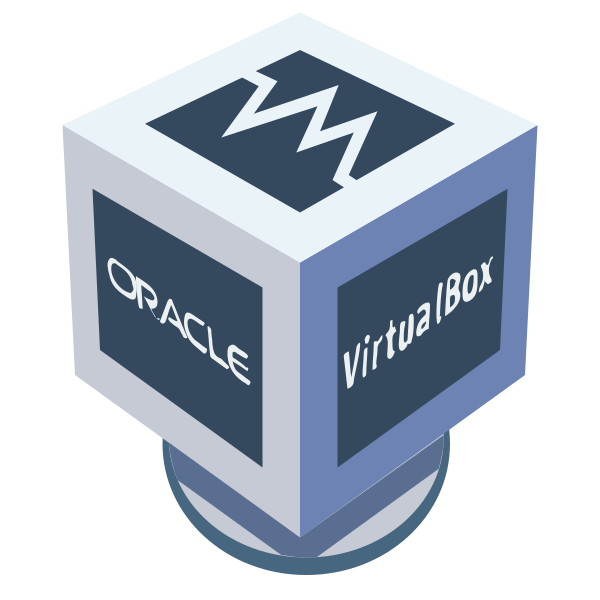
\includegraphics[width=0.3\textwidth, keepaspectratio]{image/Tools/virtualbox-logo.png}
        \caption[Virtual Machine Logo]{Virtual Machine Logo\footnotemark}
        \label{fig:Virtual Machine_logo}
        \footnotetext{\url{https://www.vmware.com/topics/virtual-machine}}
    \end{figure}
    \FloatBarrier
    \qquad Virtual Machine (VM) คือ ซอฟต์แวร์ที่สร้างสภาพแวดล้อมเสมือนบนคอมพิวเตอร์จริง ซึ่งช่วยให้สามารถรันระบบปฏิบัติการและแอปพลิเคชันต่าง ๆ ได้อย่างแยกจากกัน VM ช่วยให้ผู้ใช้สามารถทดสอบซอฟต์แวร์ในสภาพแวดล้อมที่ปลอดภัย และสามารถจัดการทรัพยากรของระบบได้อย่างมีประสิทธิภาพ
\subsection{PostgreSQL}
    \begin{figure}[ht]
        \centering
        
\includegraphics[width=0.4\textwidth, keepaspectratio]{image/Tools/postgresql-logo.png}
        \caption[PostgreSQL Logo]{PostgreSQL Logo\footnotemark}
        \label{fig:postgresql_logo}
        \footnotetext{\url{https://www.postgresql.org/}}
    \end{figure}
    \FloatBarrier
\qquad PostgreSQL คือ ระบบฐานข้อมูลแบบ Relational Database Management System (RDBMS) ที่เป็นโอเพนซอร์ส มีความสามารถในการจัดการข้อมูลที่มีความซับซ้อน รวมถึงการจัดการข้อมูลที่มีความสัมพันธ์กัน

\subsection{MinIO}
    \begin{figure}[ht]
        \centering
        
\includegraphics[width=0.4\textwidth, keepaspectratio]{image/Tools/minio-logo.png}
        \caption[MinIO Logo]{MinIO Logo\footnotemark}
        \label{fig:minio_logo}
        \footnotetext{\url{https://medium.com/@dineshvarma.guduru/reading-and-writing-data-from-to-minio-using-spark-8371aefa96d2}}
    \end{figure}
    \FloatBarrier
\qquad MinIO คือ ระบบจัดเก็บข้อมูลแบบ Object Storage ที่มีความสามารถในการจัดการข้อมูลขนาดใหญ่และมีประสิทธิภาพสูง โดย MinIO ถูกออกแบบมาเพื่อรองรับการใช้งานในสภาพแวดล้อมที่ต้องการความเร็วและความน่าเชื่อถือสูง เช่น การจัดเก็บข้อมูลสำหรับแอปพลิเคชันที่ต้องการประสิทธิภาพสูง หรือการจัดเก็บข้อมูลในระบบคลาวด์

\section{\ifenglish Project plan\else แผนการดำเนินงาน\fi}

\begin{plan}{6}{2024}{10}{2025}
    \planitem{6}{2024}{6}{2024}{เลือกหัวข้อโครงการ}
    \planitem{6}{2024}{6}{2024}{เลือกอาจารย์ที่ปรึกษา}
    \planitem{6}{2024}{7}{2024}{สํารวจความต้องการของผู้ใช้}
    \planitem{6}{2024}{8}{2024}{ศึกษาระบบ}
\end{plan}

\begin{plan}{6}{2024}{10}{2025}
    \planitem{6}{2024}{10}{2024}{ออกแบบ UX/ UI และ feature ต่างๆ}
    \planitem{10}{2024}{10}{2025}{พัฒนา Frontend}
    \planitem{10}{2024}{10}{2025}{พัฒนา Backend}
    \planitem{10}{2024}{4}{2025}{ออกแบบฐานข้อมูล}
\end{plan}


\section{\ifenglish Roles and responsibilities\else บทบาทและความรับผิดชอบ\fi}
    \begin{itemize}
        \item นายคณพัฒน์ ประเพชร รับผิดชอบในการ ทําหน้าที่ในการออกแบบและพัฒนาส่วน
ติดต่อผู้ใช้ (Frontend Development) โดยรับผิดชอบออกแบบหน้าเว็บแอปพลิเคชัน ประสบการณ์
ผู้ใช้ และการพัฒนาฟังก์ชันต่างๆ
        \item นายจิรายุ จิตรเปรม รับผิดชอบในการ
        \item นายวิศรุต สาดา รับผิดชอบในการ
    \end{itemize}

\section{\ifenglish%
Impacts of this project on society, health, safety, legal, and cultural issues
\else%
ผลกระทบด้านสังคม สุขภาพ ความปลอดภัย กฎหมาย และวัฒนธรรม
\fi}
\qquad แพลตฟอร์มนี้จะสามารถช่วยให้ผู้งานมีความสะดวกในการตรวจใบงานแบบกระดาษ และมีทางเลือกในการใช้แพลตฟอร์มสําหรับการตรวจใบงานแบบกระดาษมากยิ่งขึ้น
\chapter{\ifenglish Background Knowledge and Theory\else ทฤษฎีที่เกี่ยวข้อง\fi}

\qquad การทำโครงงาน เริ่มต้นด้วยการศึกษาค้นคว้า ทฤษฎีที่เกี่ยวข้อง หรือ งานวิจัย/โครงงาน ที่เคยมีผู้นำเสนอไว้แล้ว
ซึ่งเนื้อหาในบทนี้ก็จะเกี่ยวกับการอธิบายถึงสิ่งที่เกี่ยวข้องกับโครงงาน เพื่อให้ผู้อ่านเข้าใจเนื้อหาในบทถัดๆ ไปได้ง่ายขึ้น

\section{แพลตฟอร์มที่คล้ายคลึงกัน}
  \subsection{GradeScope}
    \begin{figure}[!h]
      \centering
      
\includegraphics[width=0.6\textwidth]{image/Background/gradescope-logo.png}
      \caption[GradeScope]{GradeScope logo}
      \label{fig:gradescope_pic}
    \end{figure}
    \FloatBarrier
    \qquad GradeScope เป็นแพลตฟอร์มหนึ่งที่ออกแบบมาเพื่อช่วยแก้ปัญหาการตรวจและให้คะแนนใบงาน ข้อสอบ หรือการบ้านของนักศึกษา
    ให้เป็นไปอย่างมีประสิทธิภาพมากยิ่งขึ้น สามารถรองรับกระบวนการสอนที่มีใบงานในรูปแบบกระดาษหรือไฟล์ดิจิทัล โดยมีการแสดงผล
    ที่เป็นมิตรกับผู้ใช้ และสามารถเข้าถึงได้ผ่านอินเทอร์เน็ต แพลตฟอร์ม GradeScope มีฟังก์ชันหลักดังนี้
      \begin{enumerate}
        \item การอัปโหลดและกำหนดเกณฑ์สำหรับการตรวจใบงาน ผู้สอนสามารถอัปโหลดใบงานและข้อสอบเป็นรูปภาพหรือไฟล์ (PDF) และกำหนดเกณฑ์การให้คะแนน (Rubrics) ได้อย่างยืดหยุ่นตามความต้องการ
        \item การตรวจและให้คะแนนที่สะดวกสบาย ระบบ GradeScope ช่วยให้ผู้สอนสามารถตรวจและให้คะแนนใบงานได้อย่างรวดเร็วผ่านหน้าจอเดียว ซึ่งผู้สอนสามารถใส่คะแนนและความคิดเห็นได้ในที่เดียวกัน และปรับคะแนนหากมีการเปลี่ยนแปลงเกณฑ์การให้คะแนน
        \item การแสดงผลและวิเคราะห์คะแนน GradeScope มีระบบการแสดงผลคะแนนของนักศึกษาในรูปแบบกราฟและสถิติต่างๆ เพื่อช่วยให้ผู้สอนวิเคราะห์ผลการเรียนรู้ของนักศึกษาในกระบวนวิชาได้ง่ายขึ้น
        \item ความสะดวกในการค้นหาและการจัดเก็บข้อมูล ระบบ GradeScope ช่วยให้ผู้สอนสามารถค้นหาใบงานและข้อสอบได้ง่ายและรวดเร็ว ไม่ต้องกังวลเรื่องการสูญหายของกระดาษ และมีการจัดเก็บข้อมูลที่เป็นระบบ
      \end{enumerate}
  \subsection{Mango}
    \begin{figure}[!h]
      \centering
      
\includegraphics[width=0.4\textwidth]{image/Background/Mango-cmu.png}
      \caption[Mango]{Mango logo}
      \label{fig:mango_pic}
    \end{figure}
    \FloatBarrier
    \qquad MangoCanvas เป็นระบบ LMS ของมหาวิทยาลัยเชียงใหม่ ที่ออกแบบมาเพื่อช่วยอาจารย์ในการจัดการการเรียนการสอน โดยผู้สอนสามารถเพิ่มกระบวนวิชาและจัดการเนื้อหา เช่น การบ้านและแบบฝึกหัด รวมถึงประกาศคะแนนและติดตามความก้าวหน้าของนักศึกษาได้ ระบบมีการรองรับการนำเข้าคะแนนในรูปแบบสเปรดชีต ซึ่งสามารถใช้แม่แบบที่ระบบเตรียมไว้ให้ หลังจากที่นำเข้าคะแนน ระบบจะคำนวณค่าทางสถิติให้อัตโนมัติ และหากผู้สอนต้องการแก้ไขคะแนน สามารถทำได้ในระบบโดยไม่ต้องกลับไปแก้ในสเปรดชีต
  \subsection{MS Team}
    \begin{figure}[!h]
      \centering
      
\includegraphics[width=0.6\textwidth]{image/Background/Microsoft-Teams-Logo.png}
      \caption[Microsoft Teams]{Microsoft Teams logo}
      \label{fig:microsoft_teams_pic}
    \end{figure}
    \FloatBarrier
    \qquad Microsoft Teams เป็นแอพลิเคชั่นที่มีความหลากหลายและมีความยืดหยุ่น ช่วยให้การจัดการการเรียนการสอนออนไลน์ และการทำงานเป็นทีมเป็นไปอย่างมีประสิทธิภาพ ช่วยเพิ่มความสะดวกให้กับผู้สอนในการสื่อสาร การมอบหมายงาน และการจัดเก็บข้อมูลต่างๆ ได้ในแพลตฟอร์มเดียว

\section{User Experience and User Interface}
  \qquad UX/UI คือการออกแบบผลิตภัณฑ์ดิจิทัล เช่น เว็บไซต์หรือแอปพลิเคชัน
  โดยที่ UX (User Experience) คือประสบการณ์ของผู้ใช้โดยรวม เน้นความรู้สึกและการใช้งานที่ง่ายและมีประสิทธิภาพ
  ส่วน UI (User Interface) คือส่วนที่ผู้ใช้มองเห็นและโต้ตอบด้วย เช่น ปุ่ม, สี, และการจัดวาง เพื่อให้ผลิตภัณฑ์นั้นดูสวยงามและน่าใช้
  \subsection{User-Centered Design (UCD)}
    \begin{figure}[h!]
      \begin{center}
        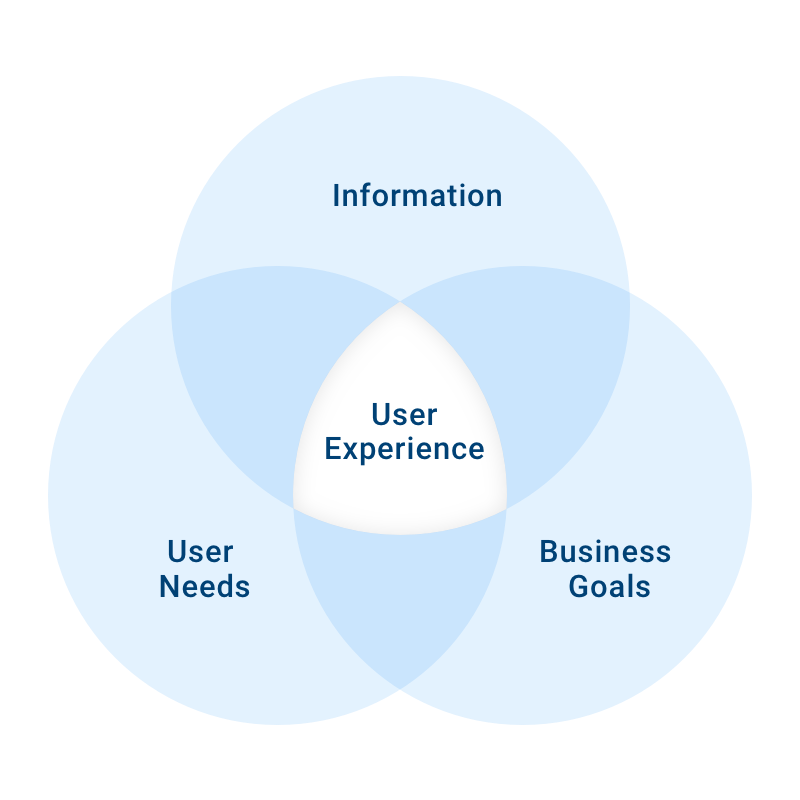
\includegraphics[scale=0.25]{image/Background/UDC.png}
      \end{center}
      \caption[User-Centered Design]{How to design in User-Centered Way}
      \label{fig:udc_pic}
    \end{figure}
    \FloatBarrier
    \qquad เป็นหลักการการออกแบบที่จัดระดับความสําคัญของความต้องการและความชอบของผู้ใช้งานตลอดกระบวนการออกแบบ โดยการทําความเข้าใจผู้ใช้เป้าหมายและบริบทของผู้ใช้ เพื่อสร้างเว็บแอพพลิเคชั่นที่ใช้งาน ง่ายมีประสิทธิภาพในการใช้งานโดยทั่วไปหลักการนี้จะเกี่ยวข้องกับการออกแบบซํ้าๆเช่น การวิจัยผู้ใช้ การสร้างต้นแบบ และการทดสอบการใช้งานเพื่อปรับปรุงประสบการณ์ของผู้ใช้อย่างต่อเนื่อง \cite{UCD1}\cite{UCD2}

  \subsection{Jakob’s Law}
    \qquad เป็นหลักการการออกแบบว่าด้วยการพัฒนาหรือปรับปรุงผลิตภัณฑ์ไม่ว่าจะเป็นสิ่งของ หรือบนเว็บไซต์
    แอพพลิเคชั่นจากความคุ้นเคยเดิมของผู้ใช้ ให้สามารถใช้งานผลิตภัณฑ์ได้ง่ายและสะดวกมากขึ้นโดยที่ไม่ต้องเริ่ม
    เรียนรู้การใช้งานใหม่อีกครั้ง โดยจะใช้รูปแบบ UI ที่ผู้ใช้คุ้นเคยเพื่อไม่ให้ผู้ใช้ต้องปรับตัวใหม่หรือการจัดองค์ประกอบของส่วนต่างๆ
    ในหน้า layout ให้เหมาะสม ไม่พยายามเปลี่ยนแปลงประสบการณ์ของผู้ใช้มากจนเกินไป ซึ่งความสอดคล้องตรงนี้จะช่วยให้
    ผู้ใช้รู้สึกสบายและมั่นใจในการใช้ผลิตภัณฑ์มากขึ้น เมื่อองค์ประกอบบนเว็บไซต์ต้องทํางานสอดคล้องกับความคาดหวังของผู้ใช้งาน \cite{Jakob}

\section{Platform Development}
  \subsection{Sprints}
    \begin{figure}[!ht]
      \centering
      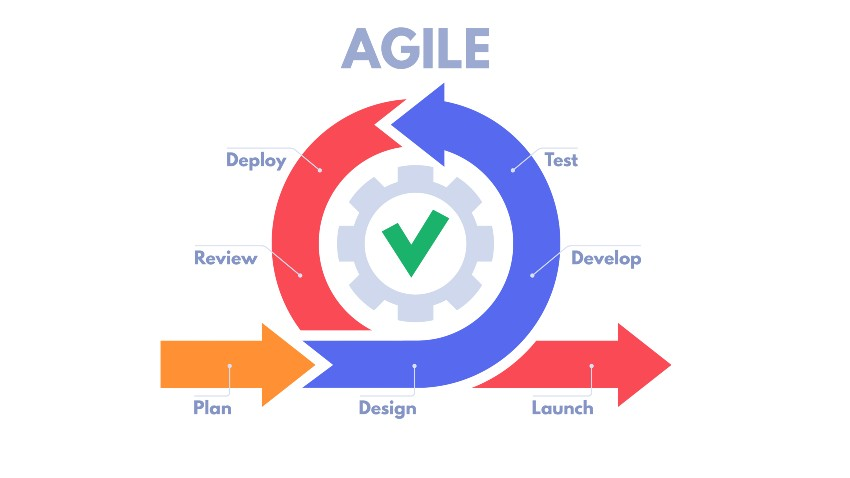
\includegraphics[width=0.8\textwidth]{image/Background/Sprints.jpg}
      \caption[Sprints]{Sprints concept}
      \label{fig:sprints_pic}
    \end{figure}
    \FloatBarrier
    \qquad Sprints คือ ช่วงเวลาที่กำหนดไว้ล่วงหน้าในกระบวนการพัฒนาซอฟต์แวร์แบบ Agile
    ซึ่งทีมพัฒนาจะทำงานร่วมกันเพื่อสร้างและส่งมอบฟีเจอร์ หรือส่วนประกอบของซอฟต์แวร์ในระยะเวลาที่กำหนด
    โดยที่ทั่วไป Sprints จะมีระยะเวลาประมาณ 1-4 สัปดาห์ ซึ่งในแต่ละ Sprint ทีมจะวางแผนงาน
    พัฒนา ทดสอบ และส่งมอบซอฟต์แวร์ที่มีคุณภาพสูงให้กับผู้ใช้หรือลูกค้าได้อย่างต่อเนื่อง
    การใช้ Sprints ช่วยให้ทีมสามารถปรับตัวและตอบสนองต่อการเปลี่ยนแปลงได้อย่างรวดเร็ว
    และส่งมอบซอฟต์แวร์ที่ตรงกับความต้องการของผู้ใช้มากยิ่งขึ้น \cite{Sprint}
  \subsection{Agile}
    \begin{figure}[!ht]
      \centering
      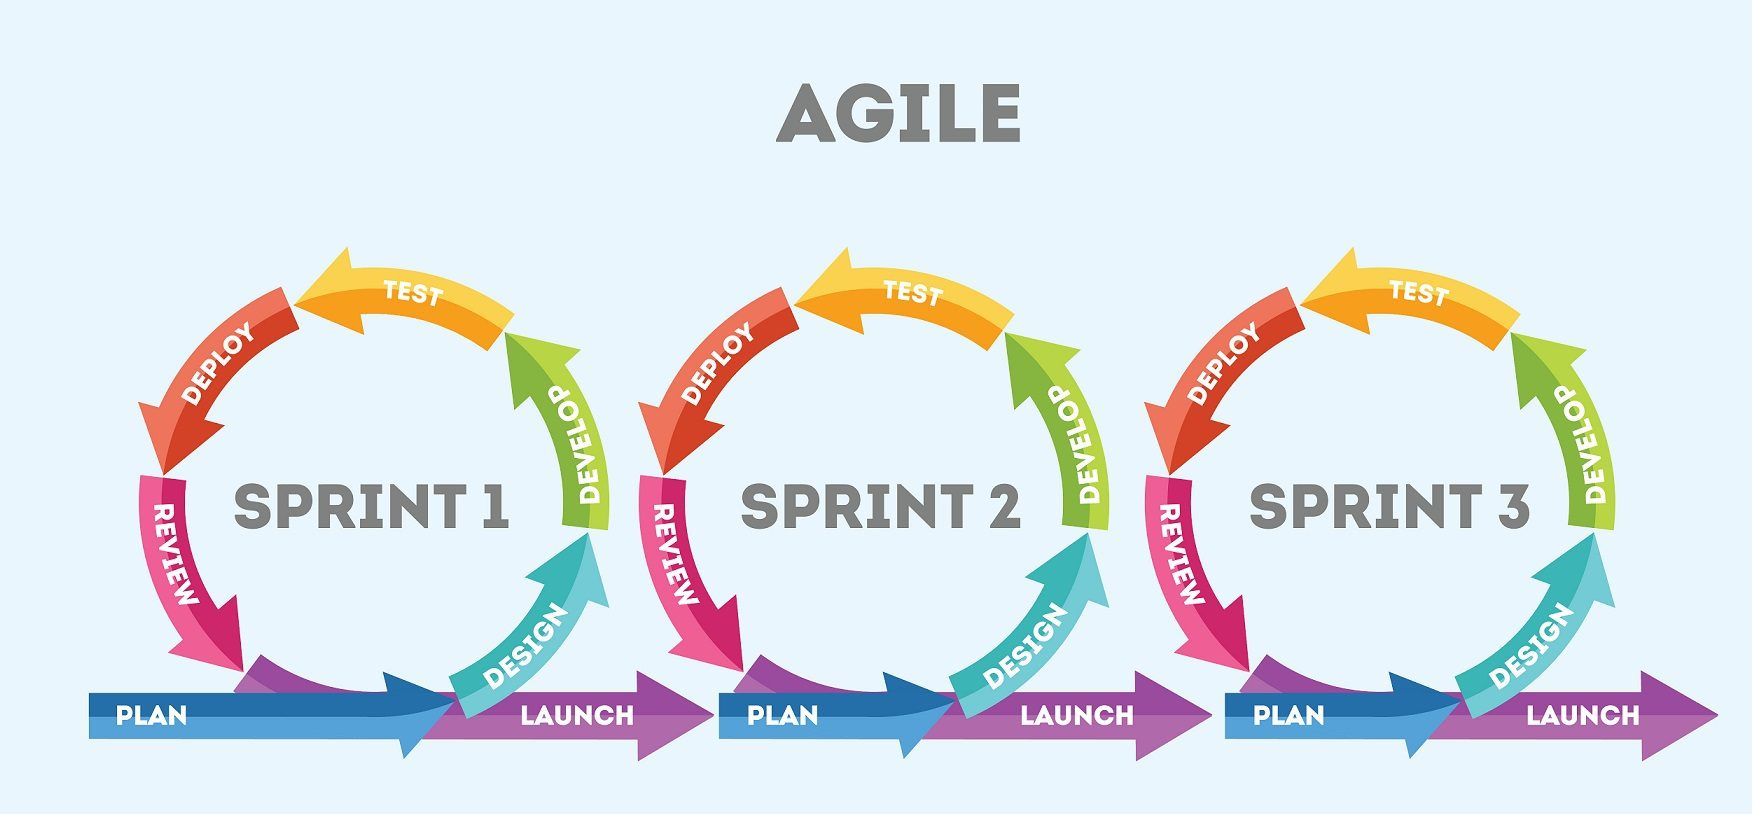
\includegraphics[width=0.8\textwidth]{image/Background/Agile-software.jpeg}
      \caption[Agile]{Agile concept}
      \label{fig:agile_pic}
    \end{figure}
    \FloatBarrier
    \qquad Agile เป็นแนวทางการพัฒนาซอฟต์แวร์ที่เน้นการทำงานร่วมกันอย่างใกล้ชิดระหว่างทีมพัฒนาและผู้มีส่วนได้ส่วนเสีย
    โดยมีการแบ่งงานออกเป็นรอบสั้น ๆ ที่เรียกว่า สปรินต์ (Sprints) ซึ่งแต่ละสปรินต์จะมีการวางแผน การพัฒนา และการทดสอบอย่างรวดเร็ว
    Agile เน้นการตอบสนองต่อการเปลี่ยนแปลงอย่างรวดเร็ว และการส่งมอบซอฟต์แวร์ที่มีคุณภาพสูงอย่างต่อเนื่อง โดยมีหลักการสำคัญดังนี้ \cite{Agile}
    \begin{enumerate}
      \item การทำงานร่วมกันระหว่างทีมพัฒนาและผู้มีส่วนได้ส่วนเสียอย่างใกล้ชิด
      \item การแบ่งงานออกเป็นรอบสั้น ๆ ที่เรียกว่า สปรินต์ (Sprints)
      \item การตอบสนองต่อการเปลี่ยนแปลงอย่างรวดเร็ว
      \item การส่งมอบซอฟต์แวร์ที่มีคุณภาพสูงอย่างต่อเนื่อง
      \item การปรับปรุงกระบวนการพัฒนาอย่างต่อเนื่อง
      \item การให้ความสำคัญกับบุคคลและปฏิสัมพันธ์มากกว่ากระบวนการและเครื่องมือ
    \end{enumerate}
  \subsection{REST API}
    \begin{figure}[!h]
      \centering
      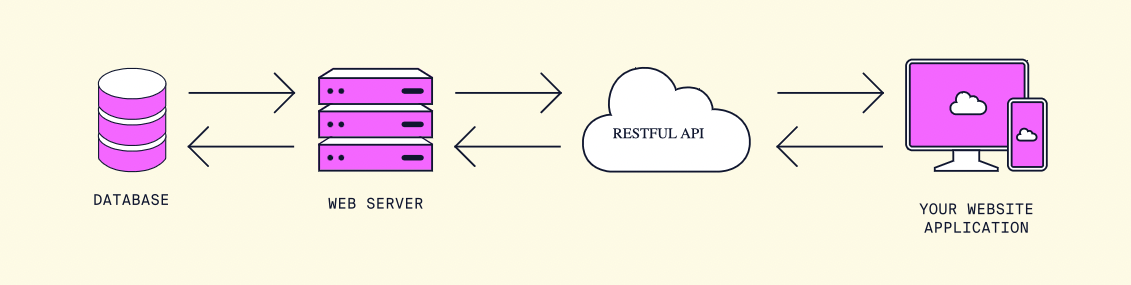
\includegraphics[width=0.8\textwidth]{image/Background/REST-API.png}
      \caption[REST API]{REST API concept}
      \label{fig:api_pic}
    \end{figure}
    \qquad REST ย่อมาจาก Representational State Transfer เป็นรูปแบบการส่งข้อมูลระหว่าง Server Client
    รูปแบบหนึ่งซึ่งอยู่บนพื้นฐานของ HTTP Protocol เป็นการสร้าง Web Service เพื่อแลกเปลี่ยน ข้อมูลกันผ่าน Application
    วิธีหนึ่งซึ่งส่งข้อมูลได้หลายชนิด ไม่ว่าจะเป็น Text, XML, JSON หรือแม้แต่ HTML ก็สามารถส่งได้ \cite{API}
    
    \qquad API ย่อมาจาก Application Programming Interface คือการเชื่อมต่อจากระบบหนึ่งไปยังอีกระบบหนึ่งเพื่อให้ซอฟต์แวร์
    ภายนอกเข้าถึงและอัพเดทข้อมูลนั้นๆได้ แต่ยังอยู่ภายในขอบเขตที่ถูกกําหนดไว้ กล่าวคือ API เป็นตัวกลางที่จะทําให้คอยรับคําสั่งต่างๆ 
    ประมวลผลและกระทําข้อมูลส่งกลับคืนไปยังคนสั่งโดยอัตโนมัติ \cite{RESTAPI}
  \subsection{Microservices}
    \begin{figure}[!h]
      \centering
      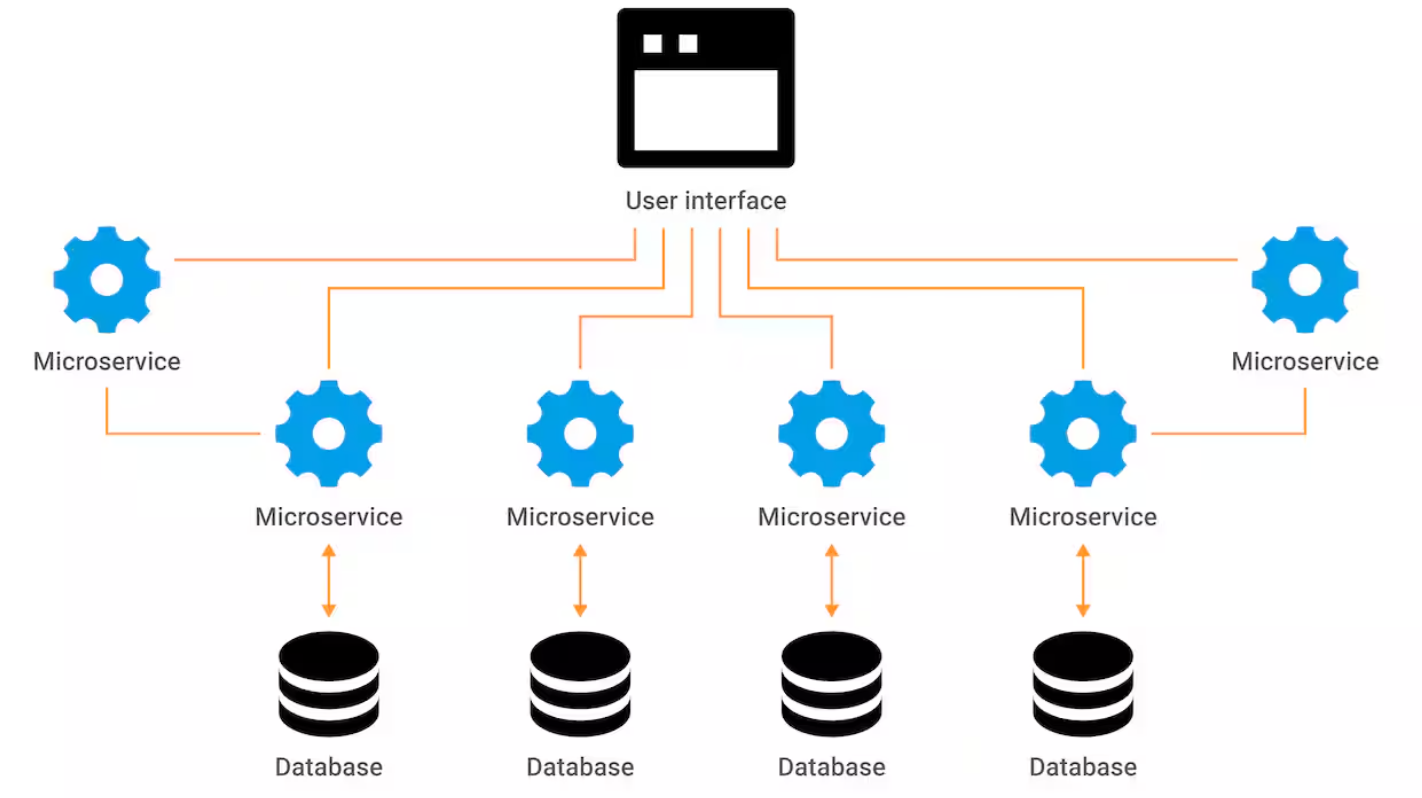
\includegraphics[width=0.8\textwidth]{image/Background/Microservices.png}
      \caption[Microservices]{Microservices concept}
      \label{fig:microservices_pic}
    \end{figure}
    \FloatBarrier
    \qquad Microservices เป็นสถาปัตยกรรมการพัฒนาซอฟต์แวร์ที่แบ่งระบบใหญ่ๆ ออกเป็นบริการเล็กๆ ที่สามารถพัฒนา
    ทดสอบ และปรับใช้ได้อย่างอิสระ โดยแต่ละบริการจะมีฟังก์ชันการทำงานเฉพาะตัวและสามารถสื่อสารกันผ่าน API 
    ได้อย่างมีประสิทธิภาพ \cite{Microservices}

  \subsection{Hexagonal Architecture}
    \begin{figure}[!h]
      \centering
      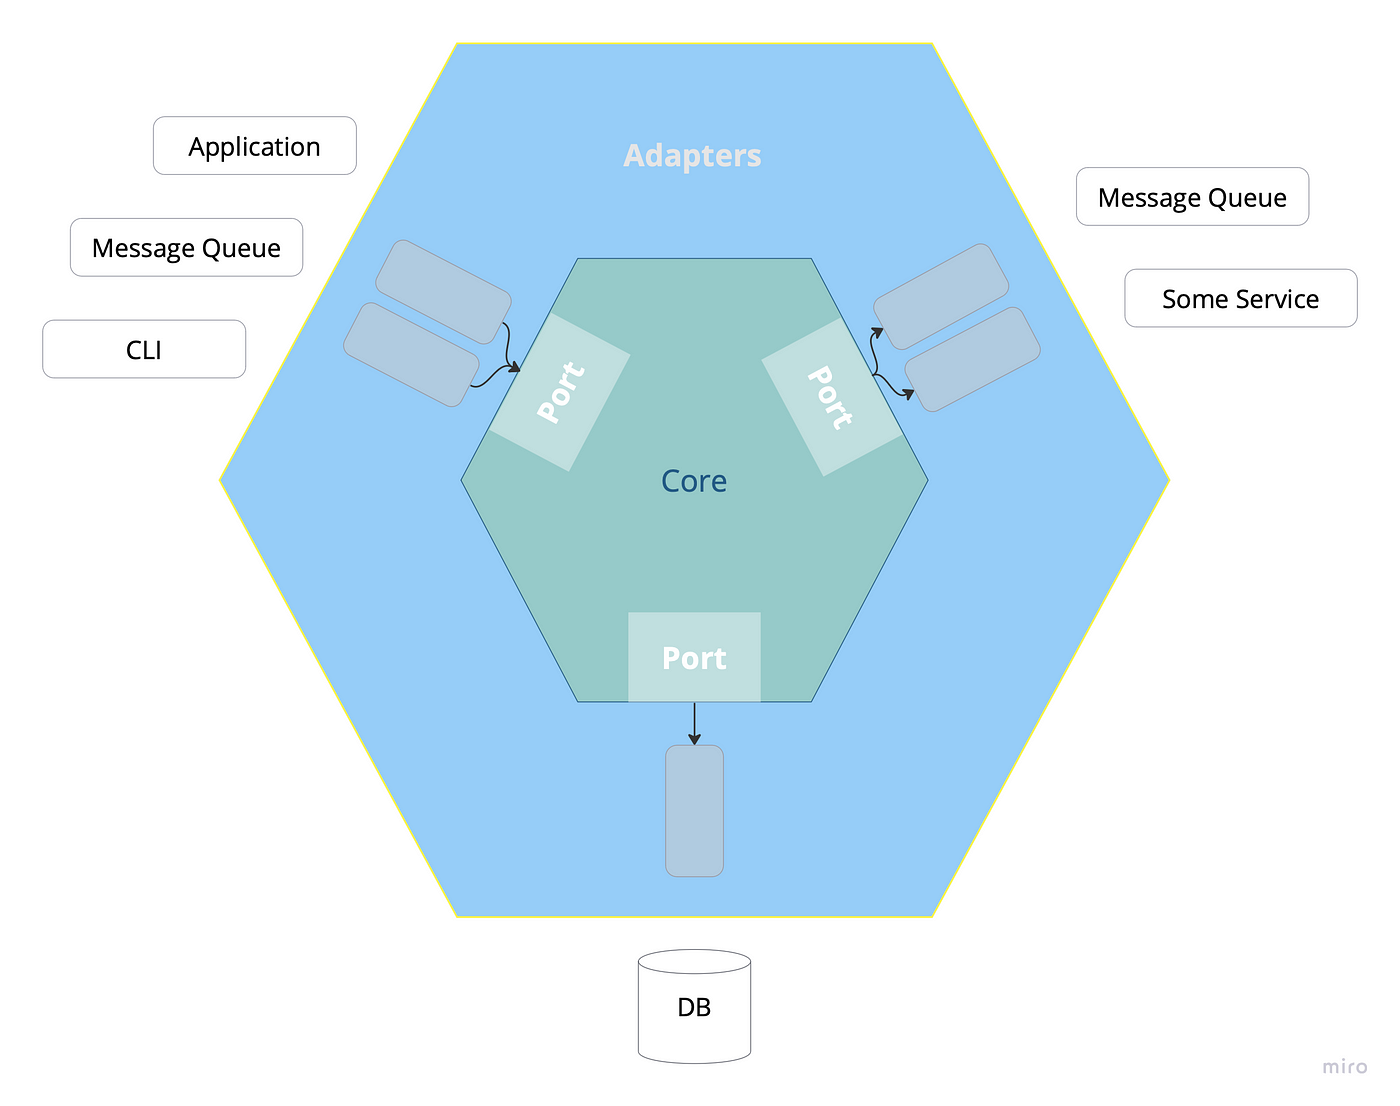
\includegraphics[width=0.6\textwidth]{image/Background/hex.png}
      \caption[Hexagonal Architecture]{โครงสร้างสถาปัตยกรรม Hexagonal}
      \label{fig:hex_pic}
    \end{figure}
    \FloatBarrier
    \qquad Hexagonal Architecture เป็น 1 ใน Code Architecture Pattern ที่เป็นที่นิยมของ Go ที่สร้างอยู่บน 2 pattern หลักๆ คือ Adaptor Pattern และ Dependency Injection  โดยองค์ประกอบหลักของ Hexagonal Architecture จะประกอบด้วยของ 3 อย่าง \cite{Hexagonal1}\cite{Hexagonal2}
    \begin{enumerate}
      \item Ports: เป็นส่วนของ Interfaces ที่กำหนดวิธีการที่แอปพลิเคชันสามารถเชื่อมต่อและติดต่อสื่อสารกับส่วนของ business logic รวมถึงการเข้าถึงทรัพยากรภายนอก โดย Ports ทำหน้าที่เป็นประตูการเชื่อมต่อระหว่าง business logic และระบบภายนอก ทำให้การเชื่อมโยงข้อมูลหรือบริการเป็นไปตามรูปแบบที่กำหนด\
      \item Adapters: เป็นส่วนที่ทำหน้าที่เชื่อมต่อกับ Ports เปรียบเสมือน "สะพาน" ที่เชื่อมโยงระหว่างทรัพยากรภายนอกจริง (เช่น ฐานข้อมูล, บริการเว็บเซอร์วิส) กับ business logic โดย Adapters จะทำหน้าที่แปลงข้อมูลระหว่าง Ports กับทรัพยากรที่ติดต่อด้วย เพื่อให้การสื่อสารระหว่าง business logic และระบบภายนอกสามารถทำงานร่วมกันได้อย่างราบรื่น
      \item Domain-centric เป็นส่วนที่อยู่ตรงกลางของ business logic และเป็นศูนย์กลางของการประมวลผลและการคำนวณต่างๆ ในแอปพลิเคชัน ทำหน้าที่จัดการตรรกะหลักของระบบโดยไม่ผูกติดกับการทำงานของระบบภายนอก เป็นศูนย์กลางของกระบวนการและกฎทางธุรกิจ (business rules) เพื่อให้ระบบมีความเป็นอิสระและแยกจากการพึ่งพาทรัพยากรภายนอก
    \end{enumerate}
    \subsection{Reverse Proxy}
    \begin{figure}[!h]
      \centering
      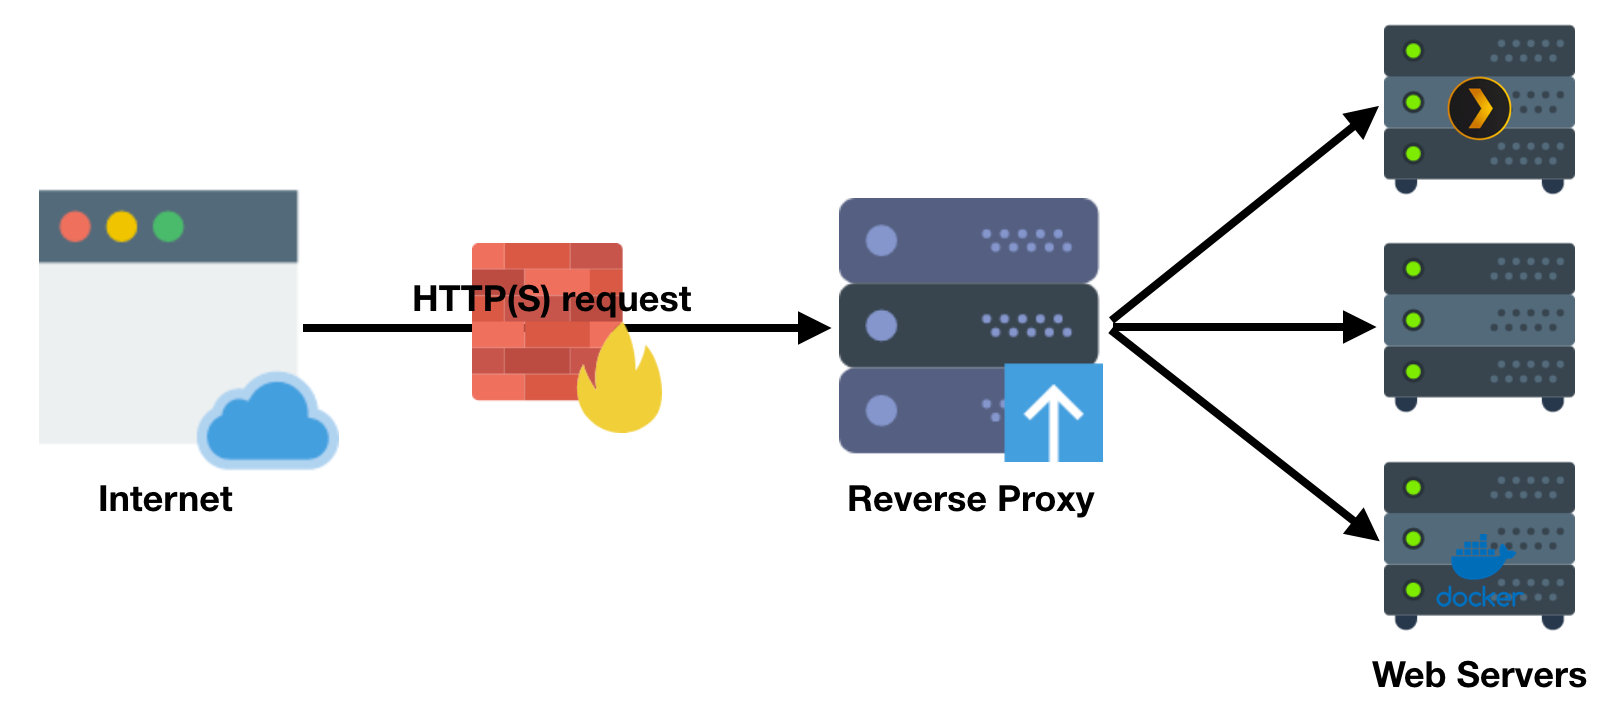
\includegraphics[width=0.6\textwidth]{image/Background/Reverse-proxy.png}
      \caption[Reverse Proxy]{Structure of Reverse Proxy}
      \label{fig:reverse_proxy_pic}
    \end{figure}
    \qquad Reverse Proxy คือ เซิร์ฟเวอร์ที่ทำหน้าที่เป็นตัวกลางระหว่างผู้ใช้ (Clients) กับเซิร์ฟเวอร์หลัก (Origin Servers)
    โดย Reverse Proxy จะรับคำขอ (Requests) จากผู้ใช้และส่งต่อไปยังเซิร์ฟเวอร์หลัก จากนั้นจะรับคำตอบ (Responses)
    จากเซิร์ฟเวอร์หลักและส่งกลับไปยังผู้ใช้ อีกครั้ง Reverse Proxy มีประโยชน์หลายประการ เช่น \cite{ReverseProxy}
    \begin{enumerate}
      \item การเพิ่มประสิทธิภาพ: Reverse Proxy สามารถทำหน้าที่เป็นตัวเก็บแคช (Cache) เพื่อเก็บข้อมูลที่ถูกเรียกใช้งานบ่อยๆ
      ซึ่งช่วยลดภาระงานของเซิร์ฟเวอร์หลักและเพิ่มความเร็วในการตอบสนองต่อผู้ใช้
      \item การกระจายโหลด: Reverse Proxy สามารถกระจายคำขอไปยังเซิร์ฟเวอร์หลักหลายๆ ตัว
      ซึ่งช่วยให้ระบบสามารถรองรับการใช้งานที่มีปริมาณมากได้อย่างมีประสิทธิภาพ
      \item ความปลอดภัย: Reverse Proxy สามารถทำหน้าที่เป็นเกราะป้องกัน (Firewall)
      โดยการกรองคำขอที่ไม่ปลอดภัยและป้องกันการโจมตีจากภายนอก
      \item การจัดการ SSL/TLS: Reverse Proxy สามารถจัดการการเข้ารหัสข้อมูลด้วย SSL/TLS
      แทนเซิร์ฟเวอร์หลัก ซึ่งช่วยลดภาระงานของเซิร์ฟเวอร์หลักและทำให้การจัดการใบรับรองดิจิทัลง่ายขึ้น
    \end{enumerate}
    
  \subsection{Tailwind CSS}
      \begin{figure}[!h]
      \centering
      
\includegraphics[width=0.6\textwidth]{image/Background/tailwind-overview.png}
      \caption{ Tailwind CSS logo}
      \label{fig:tailwind}
    \end{figure}
    \qquad Tailwind CSS คือเฟรมเวิร์ก CSS แบบ “utility-first” ที่ให้คลาสสไตล์สั้น ๆ ใช้แต่งองค์ประกอบหน้าเว็บได้อย่างรวดเร็ว โดยไม่จำเป็นต้องเขียนคลาสเฉพาะสำหรับปุ่ม/ตาราง ฯลฯ เอง เช่น การใช้ bg-yellow-200, font-bold, rounded-lg เพื่อกำหนดสีพื้นหลัง, ตัวหนา และมุมโค้งได้โดยตรงซึ่งมีประโยชน์หลายประการ เช่น \cite{Tailwind}
     \begin{enumerate}
      \item พัฒนาวิดเจ็ต/เลย์เอาต์ได้เร็ว เพราะใช้คลาสสั้นจาก Tailwind แทนเขียน CSS ใหม่ทั้งหมด
      \item รองรับการออกแบบแบบ responsive และ state (hover, focus, dark mode) ได้ง่ายผ่านระบบ variants เช่น md:bg-yellow-400 หรือ hover:bg-blue-500
    \end{enumerate}

  \subsection{MantineUI}
  \begin{figure}[!h]
    \centering
    
\includegraphics[width=0.86\textwidth]{Image/Background/mantine.png}
    \caption{Mantine logo}
  \label{fig:mantine}
  \end{figure}
    \qquad Mantine UI เป็นไลบรารีคอมโพเนนต์ React ที่มีคอมโพเนนต์พร้อมใช้งานกว่า 120 แบบ (เช่น Button, Modal, Tabs, Table) และรองรับธีม แสง/มืด (Light/Dark) โดยออกแบบมาให้สร้างเว็บแอปได้เร็วขึ้น ซึ่งมีประโยชน์หลายประการ เช่น \cite{Mantine}
 \begin{enumerate}
      \item มีคอมโพเนนต์พร้อมใช้งานหลากหลาย ทำให้เราสามารถใช้คอมโพเนนต์สำเร็จรูปแทนการสร้างเองจากศูนย์
      \item รองรับ custom styling และ integration กับ React Hooks เช่น useClipboard, useForm, useDisclosure ซึ่งช่วยจัดการโมดัล/สถานะ/อินเทอร์แอคชั่นได้ง่าย
      \item รองรับธีมแบบ Dark/Light สลับได้อัตโนมัติ รวมถึงปรับแต่งธีม (สี ฟอนต์ เงา) ได้ง่าย
    \end{enumerate}

  \subsection{App Router}
    \begin{figure}[!h]
      \centering
      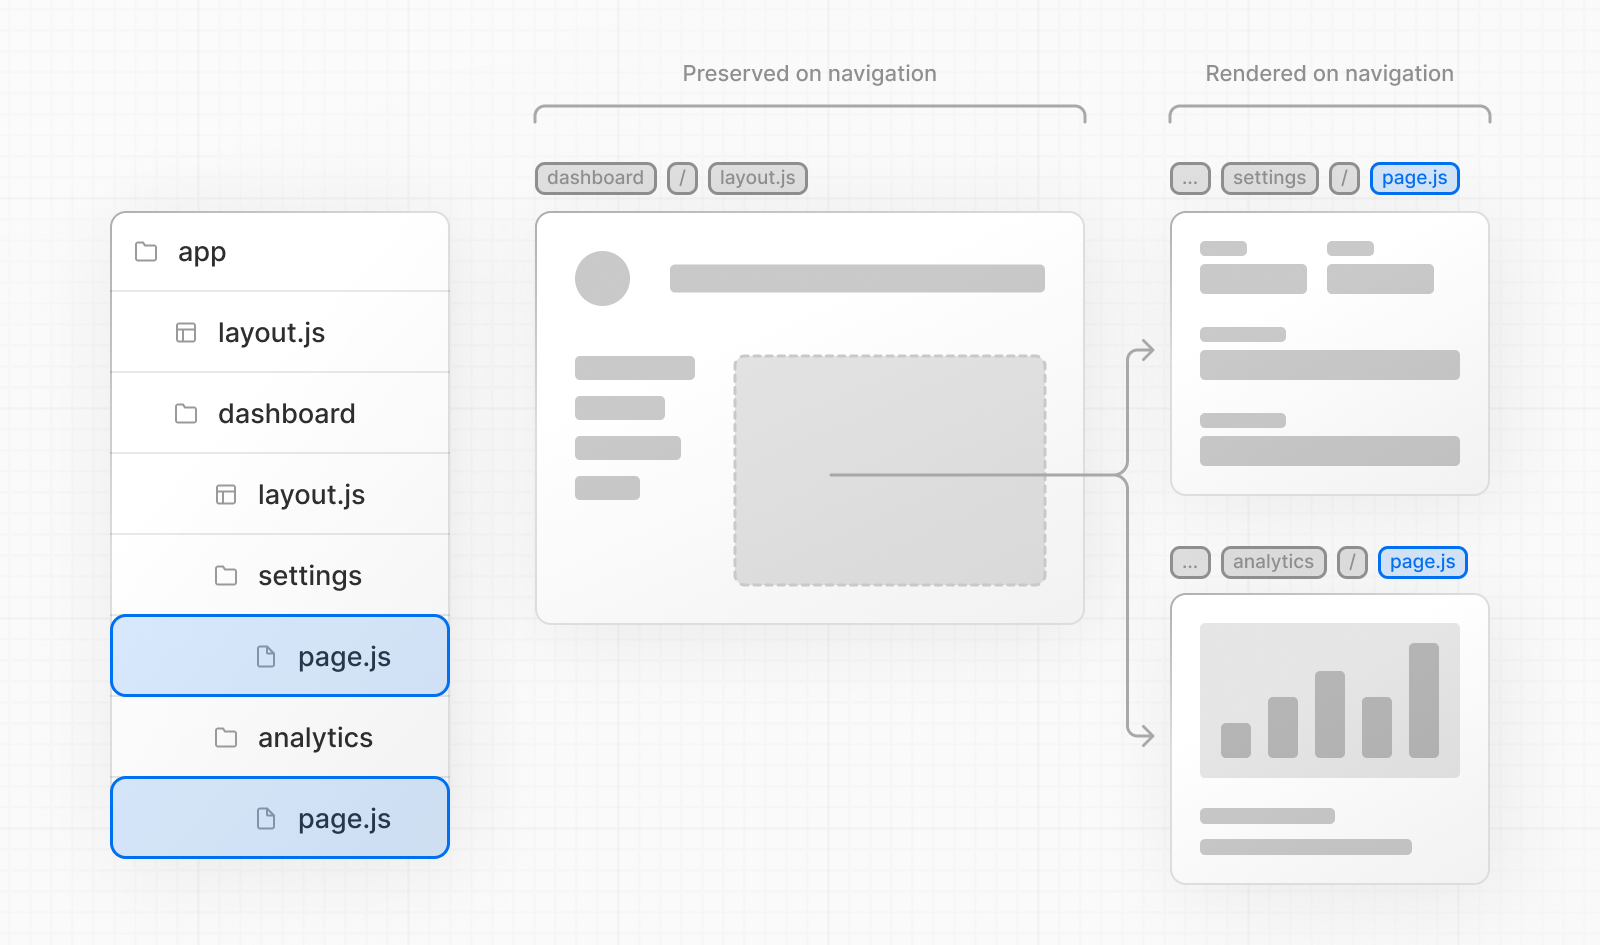
\includegraphics[width=0.6\textwidth]{image/Background/app-router.png}
      \caption[App Router]{โครงสร้างของ App Router}
      \label{fig:app_router_pic}
    \end{figure}
    \FloatBarrier
    \qquad App Router เป็นเครื่องมือที่ช่วยในการจัดการเส้นทาง (Routing) ของแอปพลิเคชันเว็บ
    ซึ่งช่วยให้การนำทางระหว่างหน้าและส่วนต่างๆ ของแอปพลิเคชันเป็นไปอย่างราบรื่นและมีประสิทธิภาพ โดย App Router
    จะทำหน้าที่จับคู่ URL ที่ผู้ใช้ร้องขอเข้ากับคอมโพเนนต์หรือหน้าที่เหมาะสมในแอปพลิเคชัน ซึ่งช่วยให้ผู้พัฒนาสามารถสร้างแอปพลิเคชัน
    ที่มีโครงสร้างที่ชัดเจนและง่ายต่อการดูแลรักษา นอกจากนี้ App Router ยังสนับสนุนฟีเจอร์ต่างๆ เช่น การจัดการสถานะของหน้า
    การส่งผ่านพารามิเตอร์ และการจัดการเส้นทางแบบไดนามิก ทำให้ผู้ใช้สามารถเข้าถึงเนื้อหาต่างๆ ได้อย่างรวดเร็วและสะดวกสบาย
    \cite{AppRouter} \cite{Routing}

  \subsection{Json Web Token (JWT)}
    \begin{figure}[!h]
      \centering
      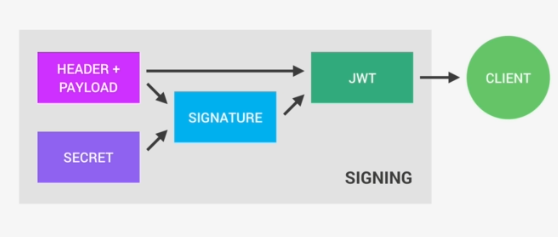
\includegraphics[width=0.6\textwidth]{image/Background/JWT.png}
      \caption[JWT]{โครงสร้างของ Json Web Token (JWT)}
      \label{fig:jwt_pic}
    \end{figure}
    \FloatBarrier
    \qquad JWT[?]เป็นมาตรฐานแบบเปิด (RFC 7519) ที่กําหนดรูปแบบข้อมูลที่มีขนาดเล็กและสามารถตรวจสอบได้ในตัวเอง
    เพื่อใช้ในการส่งข้อมูลระหว่างฝ่ายต่างๆ อย่างปลอดภัยในรูปแบบของ JSON ข้อมูลนี้สามารถตรวจสอบและเชื่อถือได้
    เนื่องจากมีการลงนามดิจิทัล (Digitally signed) \cite{JWT}
  
  \subsection{Rubric}
    \begin{figure}[!h]
      \centering
      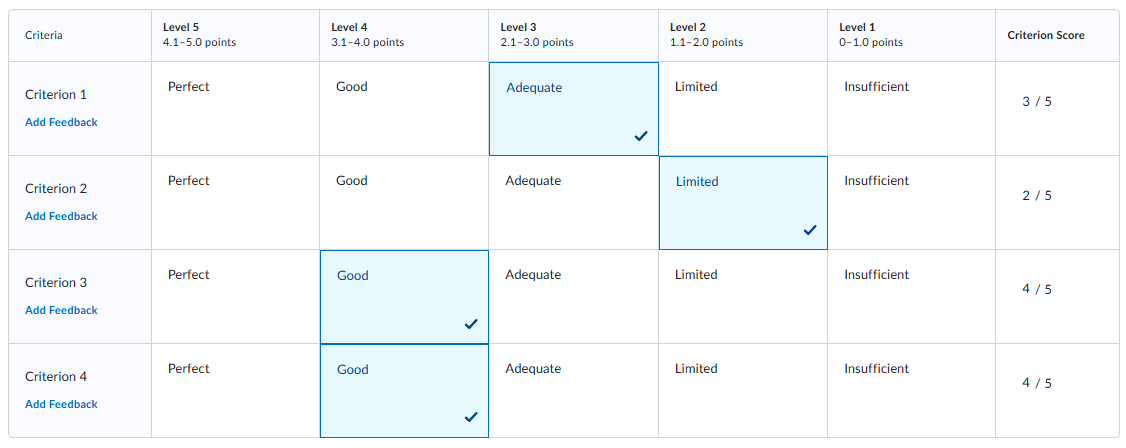
\includegraphics[width=0.8\textwidth]{image/Background/Rubrics.png}
      \caption[Rubric]{Rubric concept}
      \label{fig:rubric_pic}
    \end{figure}
    \FloatBarrier
    \qquad Rubric คือ เครื่องมือที่ใช้ในการประเมินผลการเรียนรู้ของนักศึกษา
    โดยการกำหนดเกณฑ์และระดับคะแนนสำหรับแต่ละองค์ประกอบของงานที่นักศึกษาต้องทำ
    ซึ่งช่วยให้การประเมินเป็นไปอย่างมีมาตรฐานและเป็นธรรม Rubric มักประกอบด้วย
    รายละเอียดของเกณฑ์การประเมินในแต่ละระดับคะแนน เช่น ดีมาก ดี ปานกลาง และต้องปรับปรุง
    ซึ่งช่วยให้นักศึกษาเข้าใจถึงความคาดหวังและสามารถปรับปรุงผลงานของตนได้อย่างมีประสิทธิภาพ \cite{Rubric}

\section{Database System}
  \qquad ระบบฐานข้อมูล (Database System) หมายถึงโครงสร้างสารสนเทศที่ประกอบด้วย รายละเอียดของข้อมูลที่เกี่ยวข้องกัน
  ที่จะนำมาใช้ในระบบต่างๆ ร่วมกัน ซึ่งผู้ใช้สามารถจัดการกับ ข้อมูลได้ในลักษณะต่างๆ ทั้งเพิ่ม ลบ หรือแก้ไข
  ตลอดจนการเรียกดูข้อมูลส่วนใหญ่จะเป็นการประยุกต์นำเอาระบบคอมพิวเตอร์เข้ามาช่วยในการจัดการฐานข้อมูลระบบฐานข้อมูล
  มีคําศัพท์ต่างๆที่เกี่ยวข้องดังนี้ \cite{DataBaseSystem}
  \subsection{Entity}
    \qquad Entity คือ สิ่งที่สามารถระบุได้อย่างชัดเจน เช่น บุคคล สถานที่ สิ่งของ เหตุการณ์ หรือแนวคิด ซึ่งมีความสำคัญในบริบท
    ของระบบฐานข้อมูล โดย Entity จะถูกแทนด้วยตาราง (Table) ในฐานข้อมูล และแต่ละแถว (Row) ในตารางจะเป็นการแสดงถึง
    ตัวอย่างเฉพาะของ Entity นั้นๆ เช่น ในระบบฐานข้อมูลของมหาวิทยาลัย "นักศึกษา" อาจเป็น Entity หนึ่ง โดยแต่ละแถว
    ในตารางนักศึกษาจะเป็นการแสดงถึงนักศึกษาแต่ละคนที่มีข้อมูลเฉพาะตัว เช่น ชื่อ รหัสนักศึกษา และวันเกิด \cite{Entity}
  \subsection{Attribute}
    \qquad Attribute คือ คุณสมบัติหรือลักษณะเฉพาะของ Entity ที่ใช้ในการอธิบายหรือระบุข้อมูลเพิ่มเติมเกี่ยวกับ Entity นั้นๆ
    ในระบบฐานข้อมูล Attribute จะถูกแทนด้วยคอลัมน์ (Column) ในตาราง และแต่ละคอลัมน์จะเก็บข้อมูลเฉพาะเจาะจงเกี่ยวกับ
    Entity ตัวอย่างเช่น ในตารางนักศึกษา Attribute อาจประกอบด้วย ชื่อ (name), รหัสนักศึกษา (student ID),
    วันเกิด (date of birth) เป็นต้น ซึ่งแต่ละ Attribute จะมีค่าที่แตกต่างกันสำหรับแต่ละแถวในตาราง \cite{Attribute}
  \subsection{Relationship}
    \qquad Relationship คือ ความสัมพันธ์ระหว่าง Entity ต่างๆ ในระบบฐานข้อมูล ซึ่งแสดงถึงวิธีที่ Entity เหล่านั้นเชื่อมโยง
    หรือมีปฏิสัมพันธ์กัน โดย Relationship จะถูกแทนด้วยตารางความสัมพันธ์ (Relationship table)
    หรือคอลัมน์ในตารางที่เชื่อมโยง Entity ต่าง ๆ เข้าด้วยกัน ตัวอย่างเช่น ในระบบฐานข้อมูลของมหาวิทยาลัย อาจมี
    Relationship ระหว่าง Entity "นักศึกษา" กับ "หลักสูตร" ที่แสดงว่านักศึกษาแต่ละคนสามารถลงทะเบียนเรียนในหลักสูตรต่างๆ ได้อย่างไร
  \subsection{Primary Key}
    \qquad Primary Key คือ คอลัมน์หรือชุดของคอลัมน์ในตารางฐานข้อมูลที่มีคุณสมบัติพิเศษที่ใช้ในการระบุแถว (Row)
    แต่ละแถวในตารางอย่างไม่ซ้ำกัน Primary Key จะต้องมีค่าที่ไม่ซ้ำกัน (Unique) และไม่เป็นค่า null (Not null)
    ในแต่ละแถวของตาราง ซึ่งช่วยให้สามารถเข้าถึงและจัดการข้อมูลได้อย่างมีประสิทธิภาพ นอกจากนี้ Primary Key
    ยังช่วยในการสร้างความสัมพันธ์ระหว่างตารางต่างๆ ในฐานข้อมูลผ่านการใช้คีย์นอก (Foreign key) ที่เชื่อมโยงกับ
    Primary Key ของตารางอื่นๆ \cite{PrimaryKey}
  \subsection{Foreign Key}
    \qquad Foreign Key คือ คอลัมน์หรือชุดของคอลัมน์ในตารางฐานข้อมูลที่ใช้เพื่อสร้างความสัมพันธ์ระหว่างตารางต่างๆ โดย
    Foreign Key จะอ้างอิงถึง Primary Key ของตารางอื่น ซึ่งช่วยให้สามารถเชื่อมโยงข้อมูลระหว่างตารางได้อย่างมีประสิทธิภาพ
    Foreign Key ช่วยในการรักษาความสมบูรณ์ของข้อมูล (Data integrity) โดยการบังคับใช้ข้อจำกัดที่ทำให้ค่าของ
    Foreign Key ต้องตรงกับค่าของ Primary Key ในตารางที่อ้างอิง หรือเป็นค่า Null เท่านั้น \cite{ForeignKey}
  \subsection{Relational Database Management System (RDBMS)}
    \qquad RDBMS เป็นระบบจัดการฐานข้อมูลที่ใช้โครงสร้างแบบตาราง (table) เพื่อจัดเก็บข้อมูล โดยแต่ละตารางจะประกอบด้วย
    แถว (Row) และคอลัมน์ (Column) ซึ่งช่วยให้การจัดการและการเข้าถึงข้อมูลเป็นไปอย่างมีประสิทธิภาพ RDBMS ใช้ภาษา SQL
    (Structured Query Language) ในการสร้าง แก้ไข และดึงข้อมูลจากฐานข้อมูล นอกจากนี้ RDBMS ยังสนับสนุนความสัมพันธ์
    ระหว่างตารางต่างๆ ผ่านคีย์หลัก (Primary Key) และคีย์นอก (Foreign Key) ซึ่งช่วยให้สามารถเชื่อมโยงข้อมูลระหว่างตาราง
    ได้อย่างมีประสิทธิภาพ \cite{RDBMS}

\section{Storage}
  \subsection{Object Storage}
    \qquad Object Storage คือ รูปแบบการจัดเก็บข้อมูลที่ใช้ในการจัดการและเก็บข้อมูลในรูปแบบของวัตถุ (Objects)
    ซึ่งแต่ละวัตถุจะประกอบด้วยข้อมูล (Data) และเมตาดาต้า (Metadata) ที่อธิบายลักษณะและคุณสมบัติของข้อมูลนั้นๆ 
    Object Storage มีความยืดหยุ่นสูง สามารถจัดเก็บข้อมูลได้หลากหลายประเภท เช่น ไฟล์ภาพ วิดีโอ เอกสาร และข้อมูลอื่นๆ
    โดยไม่จำเป็นต้องมีโครงสร้างตารางเหมือนกับฐานข้อมูลแบบดั้งเดิม นอกจากนี้ Object Storage ยังมีความสามารถในการขยายตัว
    (Scalability) ที่ดี ทำให้สามารถรองรับปริมาณข้อมูลที่เพิ่มขึ้นได้อย่างมีประสิทธิภาพ \cite{ObjectStorage}
  \subsection{Metadata}
    \qquad Metadata คือ ข้อมูลที่อธิบายลักษณะและคุณสมบัติของข้อมูลอื่นๆ ซึ่งช่วยให้สามารถจัดการ ค้นหา และใช้งานข้อมูล
    ได้อย่างมีประสิทธิภาพ \cite{Metadata}
  \subsection{Bucket}
    \qquad Bucket คือ โครงสร้างหลักที่ใช้ในการจัดเก็บข้อมูลไฟล์ต่างๆ ในระบบจัดเก็บข้อมูลแบบอ็อบเจ็กต์ โดย Bucket
    ทำหน้าที่เป็นที่เก็บข้อมูลที่มีการจัดระเบียบและแยกประเภทอย่างชัดเจน ซึ่งช่วยให้การจัดการและการเข้าถึงข้อมูลเป็นไปอย่าง
    มีประสิทธิภาพ ในแต่ละ Bucket สามารถเก็บวัตถุ (Objects) ได้หลากหลายประเภท เช่น ไฟล์ภาพ วิดีโอ เอกสาร
    และข้อมูลอื่นๆ นอกจากนี้ Bucket ยังสามารถกำหนดสิทธิ์การเข้าถึงข้อมูลได้อย่างละเอียด เพื่อควบคุมการใช้งานและ
    รักษาความปลอดภัยของข้อมูล \cite{Bucket}

\section{Optical Character Recognition (OCR)}
  \qquad Optical Character Recognition (OCR) คือ เทคโนโลยีที่ใช้ในการแปลงภาพตัวอักษรที่ถูกสแกนหรือ
  ถ่ายภาพมาให้อยู่ในรูปแบบดิจิทัลที่สามารถแก้ไขและค้นหาได้ OCR ทำงานโดยการวิเคราะห์ภาพเพื่อระบุและแยกแยะตัวอักษร
  จากนั้นจึงแปลงตัวอักษรเหล่านั้นเป็นข้อความที่สามารถนำไปใช้ในโปรแกรมประมวลผลคำหรือฐานข้อมูลได้ 
  เทคโนโลยี OCR มีการใช้งานอย่างแพร่หลายในหลายๆ ด้าน เช่น การแปลงเอกสารกระดาษเป็นไฟล์ดิจิทัล 
  การสแกนบัตรประชาชน หรือการอ่านป้ายทะเบียนรถยนต์ เป็นต้น \cite{OCR}
  \subsection{Tesseract OCR}
    \qquad Tesseract OCR เป็นซอฟต์แวร์โอเพนซอร์สที่ใช้สำหรับการรู้จำอักขระด้วยแสง 
    (Optical Character Recognition - OCR) ซึ่งพัฒนาโดย Google Tesseract
    มีความสามารถในการแปลงภาพของตัวอักษรที่ถูกสแกนหรือถ่ายภาพมาให้อยู่ในรูปแบบดิจิทัลที่สามารถแก้ไขและค้นหาได้
    ซอฟต์แวร์นี้รองรับหลายภาษาและสามารถทำงานกับรูปแบบภาพต่างๆ เช่น JPEG, PNG, TIFF เป็นต้น Tesseract OCR
    มีการใช้งานอย่างแพร่หลายในหลายๆ ด้าน เช่น การแปลงเอกสารกระดาษเป็นไฟล์ดิจิทัล การสแกนบัตรประชาชน
    หรือการอ่านป้ายทะเบียนรถยนต์ เป็นต้น โดยข้อดีของ Tesseract OCR มีดังนี้ \cite{Tesseract}
    \begin{enumerate}
      \item เป็นซอฟต์แวร์โอเพนซอร์สที่สามารถใช้งานได้ฟรี
      \item รองรับหลายภาษาและรูปแบบภาพต่างๆ
      \item มีความแม่นยำในการรู้จำอักขระสูง
      \item สามารถปรับแต่งและขยายความสามารถได้ตามความต้องการของผู้ใช้
    \end{enumerate}

\section{Third section}
Section 3 text. The dielectric constant\index{dielectric constant}
at the air-metal interface determines
the resonance shift\index{resonance shift} as absorption or capture occurs
is shown in Equation~\eqref{eq:dielectric}:

\begin{equation}\label{eq:dielectric}
k_1=\frac{\omega}{c({1/\varepsilon_m + 1/\varepsilon_i})^{1/2}}=k_2=\frac{\omega
\sin(\theta)\varepsilon_\mathit{air}^{1/2}}{c}
\end{equation}

\noindent
where $\omega$ is the frequency of the plasmon, $c$ is the speed of
light, $\varepsilon_m$ is the dielectric constant of the metal,
$\varepsilon_i$ is the dielectric constant of neighboring insulator,
and $\varepsilon_\mathit{air}$ is the dielectric constant of air.

\section{About using figures in your report}

% define a command that produces some filler text, the lorem ipsum.
\newcommand{\loremipsum}{
  \textit{Lorem ipsum dolor sit amet, consectetur adipisicing elit, sed do
  eiusmod tempor incididunt ut labore et dolore magna aliqua. Ut enim ad
  minim veniam, quis nostrud exercitation ullamco laboris nisi ut
  aliquip ex ea commodo consequat. Duis aute irure dolor in
  reprehenderit in voluptate velit esse cillum dolore eu fugiat nulla
  pariatur. Excepteur sint occaecat cupidatat non proident, sunt in
  culpa qui officia deserunt mollit anim id est laborum.}\par}

\begin{figure}
  \centering

  \fbox{
     \parbox{.6\textwidth}{\loremipsum}
  }

  % To include an image in the figure, say myimage.pdf, you could use
  % the following code. Look up the documentation for the package
  % graphicx for more information.
  % \includegraphics[width=\textwidth]{myimage}

  \caption[Sample figure]{This figure is a sample containing \gls{lorem ipsum},
  showing you how you can include figures and glossary in your report.
  You can specify a shorter caption that will appear in the List of Figures.}
  \label{fig:sample-figure}
\end{figure}

Using \verb.\label. and \verb.\ref. commands allows us to refer to
figures easily. If we can refer to Figures
\ref{fig:walrus} and \ref{fig:sample-figure} by name in the {\LaTeX}
source code, then we will not need to update the code that refers to it
even if the placement or ordering of the figures changes.

\loremipsum\loremipsum

% This code demonstrates how to get a landscape table or figure. It
% uses the package lscape to turn everything but the page number into
% landscape orientation. Everything should be included within an
% \afterpage{ .... } to avoid causing a page break too early.
\afterpage{
  \begin{landscape}
  \begin{table}
    \caption{Sample landscape table}
    \label{tab:sample-table}

    \centering

    \begin{tabular}{c||c|c}
        Year & A & B \\
        \hline\hline
        1989 & 12 & 23 \\
        1990 & 4 & 9 \\
        1991 & 3 & 6 \\
    \end{tabular}
  \end{table}
  \end{landscape}
}

\loremipsum\loremipsum\loremipsum

\section{Overfull hbox}

When the \verb.semifinal. option is passed to the \verb.cpecmu. document class,
any line that is longer than the line width, i.e., an overfull hbox, will be
highlighted with a black solid rule:
\begin{center}
\begin{minipage}{2em}
juxtaposition
\end{minipage}
\end{center}

\section{\ifenglish%
\ifcpe CPE \else ISNE \fi knowledge used, applied, or integrated in this project
\else%
ความรู้ตามหลักสูตรซึ่งถูกนำมาใช้หรือบูรณาการในโครงงาน
\fi
}

อธิบายถึงความรู้ และแนวทางการนำความรู้ต่างๆ ที่ได้เรียนตามหลักสูตร ซึ่งถูกนำมาใช้ในโครงงาน

\section{\ifenglish%
Extracurricular knowledge used, applied, or integrated in this project
\else%
ความรู้นอกหลักสูตรซึ่งถูกนำมาใช้หรือบูรณาการในโครงงาน
\fi
}

อธิบายถึงความรู้ต่างๆ ที่เรียนรู้ด้วยตนเอง และแนวทางการนำความรู้เหล่านั้นมาใช้ในโครงงาน

\chapter{\ifproject%
\ifenglish Project Structure and Methodology\else โครงสร้างและขั้นตอนการทำงาน\fi
\else%
\ifenglish Project Structure\else โครงสร้างของโครงงาน\fi
\fi
}

\makeatletter

% \renewcommand\section{\@startsection {section}{1}{\z@}%
%                                    {13.5ex \@plus -1ex \@minus -.2ex}%
%                                    {2.3ex \@plus.2ex}%
%                                    {\normalfont\large\bfseries}}

\makeatother
%\vspace{2ex}
% \titleformat{\section}{\normalfont\bfseries}{\thesection}{1em}{}
% \titlespacing*{\section}{0pt}{10ex}{0pt}

\section{สถาปัตยกรรมระบบ}
  \qquad โครงงานนี้ได้ออกแบบสถาปัตยกรรมของระบบเป็นแบบ \textbf{Microservices} โดยบทนี้จะกล่าวถึง
    โครงสร้างของระบบทั้งหมด และอธิบายถึงแต่ละส่วนของระบบ โดยระบบจะถูกแบ่งออกเป็นส่วนย่อยๆ 
    แต่ละส่วนจะมีหน้าที่และความรับผิดชอบในการทำงานที่แตกต่างกัน

    \begin{figure}[!ht]
      \centering
      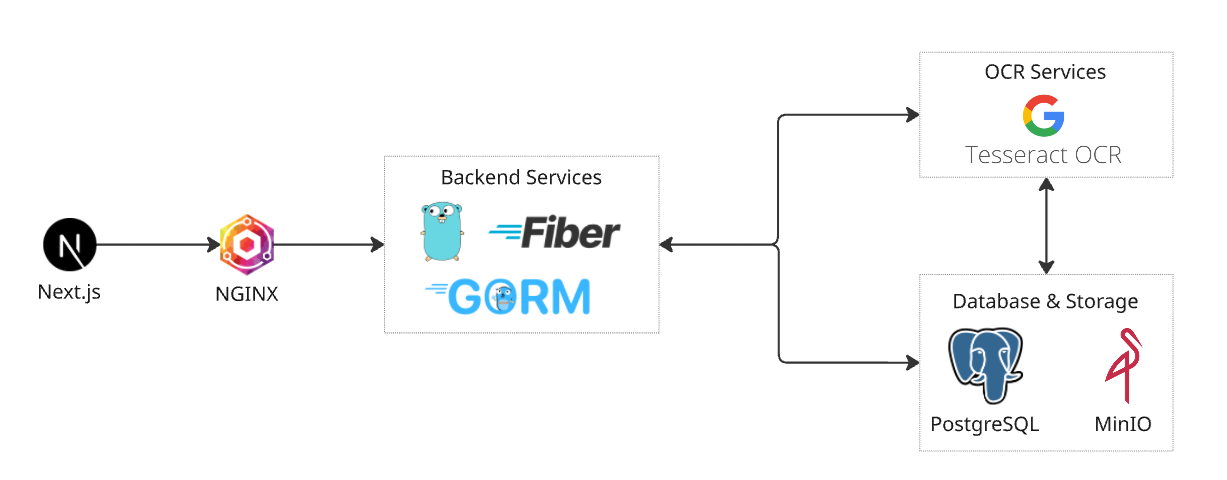
\includegraphics[width=0.8\textwidth]{image/Approach/Architecture.png}
      \caption[Architecture]{System Architecture}
      \label{fig:architecture}
    \end{figure}
    \FloatBarrier

  จากรูปที่ 3.1 แสดงถึงสถาปัตยกรรมของระบบที่ถูกแบ่งออกเป็นส่วนย่อยๆ ดังนี้
  \begin{enumerate}
    \item \textbf{Frontend} ส่วนนี้เป็นส่วนที่ทำหน้าที่ในการแสดงผลของระบบ โดยส่วนนี้จะถูกพัฒนาด้วย \textbf{Next.js}
    \item \textbf{Reverse Proxy} ส่วนนี้เป็นส่วนที่ทำหน้าที่ในการจัดการการเชื่อมต่อระหว่าง Frontend และ Backend
    โดยส่วนนั้นจะถูกพัฒนาด้วย \textbf{Nginx Proxy Manager(NPM)}
    \item \textbf{Backend} ส่วนนี้เป็นส่วนที่ทำหน้าที่ในการประมวลผลข้อมูลและให้บริการ API โดยส่วนนั้นจะถูกพัฒนาด้วย
    \textbf{Go (Golang)} และเฟรมเวิร์ก \textbf{Fiber}
    \item \textbf{OCR Service} ส่วนนี้เป็นส่วนที่ทำหน้าที่ในการประมวลผลภาพและทำการรู้จำตัวอักษร โดยส่วนนั้นจะถูกพัฒนาด้วย \textbf{Tesseract OCR}
    \item \textbf{Database and Storage} ส่วนนี้เป็นส่วนที่ทำหน้าที่ในการจัดเก็บข้อมูล โดยจะใช้ \textbf{PostgreSQL}
    เป็นฐานข้อมูลหลัก และใช้ \textbf{MinIO} สำหรับการจัดเก็บไฟล์
  \end{enumerate}

\section{โครงสร้างฐานข้อมูล (Database Schema)}
  \begin{figure}[!ht]
    \centering
    \includegraphics[width=1\textwidth]{image/Approach/Database-Schema.png}
    \caption[Database Schema]{Database Schema}
    \label{fig:database_schema}
  \end{figure}
  \FloatBarrier
  \qquad ฐานข้อมูลที่ใช้ในโครงงานนี้ คือ PostgreSQL โดยมีการออกแบบโครงสร้างฐานข้อมูล (Database Schema) เพื่อรองรับการทำงานของแพลตฟอร์มอย่างมีประสิทธิภาพ
  โดยโครงสร้างฐานข้อมูลประกอบด้วยตารางหลักๆ ดังนี้
  \begin{enumerate}
    \item \textbf{Universities} ตารางสำหรับเก็บข้อมูลรายการมหาวิทยาลัย
    \item \textbf{User Groups} ตารางสำหรับเก็บข้อมูลประเภทกลุ่มของผู้ใช้งานในแพลตฟอร์ม
    \item \textbf{Users} ตารางสำหรับเก็บข้อมูลต่างๆ ของผู้ใช้งานในแพลตฟอร์ม
    \item \textbf{Courses} ตารางสำหรับเก็บข้อมูลกระบวนวิชา
    \item \textbf{Sections} ตารางสำหรับเก็บข้อมูลลำดับตอนภายในกระบวนวิชา
    \item \textbf{Enrollment lists} ตารางสำหรับเก็บข้อมูลการลงทะเบียนของผู้ใช้งานในกระบวนวิชา
    \item \textbf{Personal Data} ตารางสำหรับเก็บข้อมูลของผู้ใช้งานในกระบวนวิชาที่ได้ลงทะเบียน
    \item \textbf{Assignments} ตารางสำหรับเก็บข้อมูลการมอบหมายงาน
    \item \textbf{Assignment Files} ตารางสำหรับเก็บข้อมูลไฟล์การมอบหมายงาน
    \item \textbf{Assignment Sections} ตารางสำหรับเก็บข้อมูลลำดับตอนภายในการมอบหมายงาน
    \item \textbf{Export Grades} ตารางสำหรับเก็บข้อมูลการส่งออกเกรด
    \item \textbf{Rubrics} ตารางสำหรับเก็บข้อมูลเกณฑ์การประเมินของใบงาน
    \item \textbf{Bounding Boxes} ตารางสำหรับเก็บข้อมูลกรอบของแต่ละใบงาน
    \item \textbf{Submissions} ตารางสำหรับเก็บข้อมูลการส่งใบงาน หรืออัพโหลดใบงาน
    \item \textbf{Submission Boxes} ตารางสำหรับเก็บข้อมูลกล่องของแต่ใบงาน ที่ใช้ในการทำ Optical Character Recognition (OCR)
    \item \textbf{Uploads} ตารางสำหรับเก็บข้อมูลการอัปโหลดไฟล์ใบงาน
    \item \textbf{Grades} ตารางสำหรับเก็บข้อมูลการให้คะแนน
  \end{enumerate}

\section{โครงสร้างระบบจัดเก็บข้อมูลแบบอ็อบเจ็กต์ (Object Storage)}
  \qquad โครงสร้างระบบจัดเก็บข้อมูลแบบอ็อบเจ็กต์ (Object Storage) ที่ใช้ในโครงงานนี้ คือ MinIO โดยมีการออกแบบโครงสร้างเพื่อรองรับการจัดเก็บไฟล์ต่างๆ
  ที่เกี่ยวข้องกับการทำงานของแพลตฟอร์ม โดยทางผู้พัฒนาได้ออกแบบไว้ในรูปแบบของ Bucket ดังนี้
  \subsection{Buckets} เป็นโครงสร้างหลักที่ใช้ในการจัดเก็บข้อมูลไฟล์ต่างๆ โดยในโครงงานนี้ได้สร้าง Bucket หลักๆ ดังนี้
    \begin{enumerate}
      \item 
      \item 
      \item 
      \item 
    \end{enumerate}

\section{Frontend}
  \qquad Frontend เป็นส่วนที่ผู้ใช้จะโต้ตอบด้วยผ่านทางเว็บเบราว์เซอร์ โดยมีหน้าที่หลักในการแสดงผลข้อมูลและรับคำสั่งจากผู้ใช้
  ซึ่งในโครงงานนี้ได้ใช้ Next.js เป็นเฟรมเวิร์กหลักในการพัฒนา และใช้ Tailwind CSS ร่วมกับ MantineUI ในการออกแบบส่วนติดต่อผู้ใช้ (User Interface)

  \section{การใช้งานพื้นฐาน}
    \qquad แพลตฟอร์มนี้ถูกออกแบบมาให้มี User Interface สำหรับผู้ใช้งาน 2 ประเภท ได้แก่ ผู้สอน (Instructor) และนักศึกษา (Student) โดยแต่ละประเภทจะมีหน้าที่และการใช้งานที่แตกต่างกัน ดังนี้
  \subsection{ผู้สอน (Instructor)}
    \par\hspace*{3em} ผู้สอนมีหน้าที่ในการสร้างและจัดการ
    \begin{enumerate}
        \item 
        \item 
        \item 
        \item 
    \end{enumerate}
  \subsection{นักศึกษา (Student)}
    \par\hspace*{3em} นักศึกษามีหน้าที่ในการ
    \begin{enumerate}
        \item 
        \item 
        \item 
        \item 
    \end{enumerate}

\include{chapters/eval}
\ifproject
\chapter{\ifenglish Conclusions and Discussions\else บทสรุปและข้อเสนอแนะ\fi}

\section{\ifenglish Conclusions\else สรุปผล\fi}

นศ. ควรสรุปถึงข้อจำกัดของระบบในด้านต่างๆ ที่ระบบมีในเนื้อหาส่วนนี้ด้วย

\section{\ifenglish Challenges\else ปัญหาที่พบและแนวทางการแก้ไข\fi}

จากการพัฒนาระบบ PaperGrader พบปัญหาสําคัญที่ส่งผลต่อประสิทธิภาพและความคล่องตัวของโครงการ
\begin{itemize}
  \item ขาดความเข้าใจเชิงลึกเกี่ยวกับระบบ ทีมพัฒนามีข้อมูลเกี่ยวกับระบบไม่มากพอ ส่งผลให้การออกแบบและพัฒนาต้องมีการเปลี่ยนแปลงบ่อยครั้ง ซึ่งกระทบต่อประสิทธิภาพของกระบวนการพัฒนา
  \item ขาดการออกแบบ UX/UI ที่เหมาะสม ทีมพัฒนาไม่ได้ออกแบบ UX/UI ให้ครอบคลุมมากพอ ส่งผลให้ระหว่างการพัฒนาต้องมีการเปลี่ยนแปลงบ่อยครั้ง ซึ่งทําให้การพัฒนาล่าช้า
  \item ความไม่แน่นอนของข้อกําหนด ข้อกําหนดของระบบมีการเปลี่ยนแปลงบ่อยครั้ง ส่งผลให้การออกแบบระบบต้องมีการปรับเปลี่ยนตาม ทําให้การพัฒนาล่าช้า
\end{itemize}
เพื่อแก้ไขปัญหาเหล่านี้ ควรมีการกําหนดข้อกําหนดให้แน่นอนตั้งแต่เริ่มต้น ใช้แนวทาง Agile ในการพัฒนา
เพื่อลดผลกระทบจากการเปลี่ยนแปลง

\section{\ifenglish%
Suggestions and further improvements
\else%
ข้อเสนอแนะและแนวทางการพัฒนาต่อ
\fi
}

เพื่อให้ระบบ PaperGrader มีประสิทธิภาพมากขึ้นในอนาคต ควรดําเนินการตามแนวทางดังต่อไปนี้:
\begin{itemize}
  \item ปรับปรุงประสิทธิภาพของระบบ OCR ในการจับคู่ใบงานกับรายชื่อนักศึกษาให้มีความแม่นยำและรวดเร็วยิ่งขึ้น
  \item พัฒนาให้การแสดงผลบนอุปกรณ์พกพารองรับได้อย่างสมบูรณ์ เพื่อความสะดวกในการใช้งานทุกแพลตฟอร์ม
  \item เพิ่มฟังก์ชันการตรวจงานแบบกลุ่ม (Group Grading) สำหรับคำตอบที่เหมือนกัน เพื่อช่วยลดระยะเวลาในการตรวจ
\end{itemize}
\fi

\bibliography{sampleReport}

\ifproject
\normalspacing
\appendix
\chapter{คู่มือการติดตั้ง}
\section{Next.js 14 (Frontend)}
  
\includegraphics[width=1\textwidth]{image/appendix/nextjs.png}
  \qquad โครงสร้างของโปรเจกต์นี้ประกอบด้วยหลายไฟล์และโฟลเดอร์ที่สําคัญสําหรับการพัฒนาและการตั้งค่าโปรเจ
กต์ โดยมีรายละเอียดดังนี้:
  \subsection{Main Files and Folders}
    \begin{enumerate}
      \item .dockerignore: ไฟล์ที่ระบุไฟล์หรือโฟลเดอร์ที่ไม่ต้องการให้Docker คัดลอกไปยัง image
      \item .env ไฟล์ที่ใช้เก็บค่าตัวแปรสภาพแวดล้อม (environment variables)สําหรับการตั้งค่าโปรเจกต์ในสภาพแวดล้อมต่างๆ
      \item .eslintrc.json: ไฟล์การตั้งค่า ESLint สําหรับการตรวจสอบและจัดรูปแบบโค้ด
      \item .gitignore: ไฟล์ที่ระบุไฟล์หรือโฟลเดอร์ที่ไม่ต้องการให้Git ติดตาม
      \item docker-compose.yml: ไฟล์การตั้งค่า Docker Compose สําหรับการจัดการ container
หลายๆ ตัว
      \item Dockerfile: ไฟล์การตั้งค่า Docker สําหรับการสร้าง Docker image
      \item next-env.d.ts: ไฟล์การตั้งค่า TypeScript สําหรับโปรเจกต์Next.js
      \item next.config.mjs: ไฟล์การตั้งค่า Next.js
      \item package.json: ไฟล์ที่เก็บข้อมูลเกี่ยวกับโปรเจกต์Node.js รวมถึง dependencies และสคริปต์
ต่างๆ
      \item postcss.config.mjs: ไฟล์การตั้งค่า PostCSS
      \item README.md: ไฟล์เอกสารสําหรับโปรเจกต
      \item tailwind.config.ts: ไฟล์การตั้งค่า Tailwind CSS
      \item tsconfig.json: ไฟล์การตั้งค่า TypeScript
    \end{enumerate}

    \subsection{Subfolders}
    \begin{enumerate}
       \item .next: โฟลเดอร์ที่เก็บไฟล์ที่ถูกสร้างขึ้นโดย Next.js หลังจากการ build
       \item app: โฟลเดอร์ที่เก็บไฟล์และโฟลเดอร์ที่เกี่ยวข้องกับการทํางานของแอปพลิเคชัน
       \item components: โฟลเดอร์ที่เก็บคอมโพเนนต์ต่างๆ ที่ใช้ในโปรเจกต์
       \item hooks: โฟลเดอร์ที่เก็บ custom hooks 
       \item store: โฟลเดอร์ที่เก็บ store
       \item public: โฟลเดอร์ที่เก็บไฟล์สาธารณะ เช่น รูปภาพ
    \end{enumerate}
\section{Installation Guide}
  \subsection{Clone the Project from GitHub}
    \qquad git clone https://github.com/jirayu123za/cpe-project-final.git
cd <repository-directory>
  \subsection{Install Dependencies}
    \qquad npm install
  \subsection{Set up Environment Variables}
    \qquad Create a .env file in the root directory and add the necessary environment variables as specified in the .env.example file.
  \subsection{Run the Development Server}
    \qquad npm run dev
  \subsection{Build for Production}
    \qquad npm run build
  \subsection{Start the Production Server}
    \qquad npm start
  \subsection{Build Docker Image (Optional)}
    \qquad npm start

\section{Golang Project (Project service)}
  \qquad รูป
  \subsection{Project Structure}
    \qquad ในส่วนข้างล่างนี้เป็นโครงสร้างของโปรเจกต์ และโฟลเดอร์ต่างๆ ที่ใช้ในโปรเจกต์นี้
    \begin{enumerate}
      \item 
      \item 
      \item 
      \item
      \item
      \item
      \item
    \end{enumerate}
  \subsection{Installation}
    \qquad ในส่วนข้างล่างนี้เป็นขั้นตอนการติดตั้งโปรเจกต์นี้
    \begin{enumerate}
      \item 
      \item 
      \item 
      \item
      \item
      \item
      \item
    \end{enumerate}
  





Text for a section in the first appendix goes here.

test ทดสอบฟอนต์ serif ภาษาไทย

\textsf{test ทดสอบฟอนต์ sans serif ภาษาไทย}

\verb+test ทดสอบฟอนต์ teletype ภาษาไทย+

\texttt{test ทดสอบฟอนต์ teletype ภาษาไทย}

\textbf{ตัวหนา serif ภาษาไทย \textsf{sans serif ภาษาไทย} \texttt{teletype ภาษาไทย}}

\textit{ตัวเอียง serif ภาษาไทย \textsf{sans serif ภาษาไทย} \texttt{teletype ภาษาไทย}}

\textbf{\textit{ตัวหนาเอียง serif ภาษาไทย \textsf{sans serif ภาษาไทย} \texttt{teletype ภาษาไทย}}}

\url{https://www.example.com/test_ทดสอบ_url}

\chapter{\ifenglish Manual\else คู่มือการใช้งานระบบ\fi}
  \qquad ข้างล่างนี้เป็นขั้นตอนการใช้งานระบบแพลตฟอร์มการตรวจใบงานแบบกระดาษ (Paper Grader) โดยแบ่งออกเป็น 2 ส่วนหลัก
  ได้แก่ ส่วนของ\textbf{ผู้สอน (Instructor)} และส่วนของ\textbf{นักเรียน (Student)}
  
\section{ส่วนของผู้สอน (Instructor)}
\section{ส่วนของนักเรียน (Student)}


%% Display glossary (optional) -- need glossary option.
\ifglossary\glossarypage\fi

%% Display index (optional) -- need idx option.
\ifindex\indexpage\fi

\begin{biosketch}
\begin{center}
  \includegraphics[width=1.5in]{mugshot.jpg}
\end{center}
Your biosketch goes here. Make sure it sits inside
the \texttt{biosketch} environment.
\end{biosketch}
\fi % \ifproject
\end{document}
